\documentclass[nochapterpage,bigchapter,linedtoc,longdoc,colorback,accentcolor=tud1c]{tudreport}
\usepackage{ngerman}
\usepackage{subfigure} 
\usepackage[stable]{footmisc}
\usepackage[ngerman]{hyperref}
\usepackage{sistyle}
\usepackage{longtable}
\usepackage{multirow}
\usepackage{booktabs}
\usepackage{graphicx}
\usepackage[backend=bibtex,style=alphabetic]{biblatex}
\bibliography{./bibtex/library}
\usepackage{amsmath}
\usepackage{caption} 
\usepackage{float}


\hypersetup{%
  pdftitle={Entwicklung und Test einer
eingebetteten Elektronik für einen
innovativen Schaltaktor},
  pdfauthor={Malte Breitenbach, Johannes Faupel, Jonas Tautz, Johanna Vetter},
  pdfsubject={Beispieltext},
  pdfview=FitH,
  pdfstartview=FitV
}

%%% Zum Tester der Marginalien %%%
  \newif\ifTUDmargin\TUDmarginfalse
  %%% Wird der Folgende Zeile einkommentiert,
  %%% werden Marginalien gesetzt.
  % \TUDmargintrue
  \ifTUDmargin\makeatletter
    \TUD@setmarginpar{2}
  \makeatother\fi
%%% ENDE: Zum Tester der Marginalien %%%

\newlength{\longtablewidth}
\setlength{\longtablewidth}{0.7\linewidth}
\addtolength{\longtablewidth}{-\marginparsep}
\addtolength{\longtablewidth}{-\marginparwidth}


% \settitlepicture{tudreport-pic}
% \printpicturesize

\title{Entwicklung und Test einer eingebetteten Elektronik für einen innovativen Schaltaktor}
\subtitle{Malte Breitenbach, Johannes Faupel, Jonas Tautz, Johanna Vetter}
%\subsubtitle{email: \textaccent{tud-design@pro-kevin.de}}
%\setinstitutionlogo[width]{TUD_sublogo}
%\uppertitleback{(\textaccent{\textbackslash uppertitleback})}
\lowertitleback{\hfill\today}
\institution{ 
Institut für Mechatronische Systeme im Maschinenbau\\
     Prof. Dr.-Ing. Stephan Rinderknecht}
%\dedication{Hier ist gen"ugend Platz\\
  %f"ur eine Widmung (\textaccent{\textbackslash dedication}).\\
  %\strut\\
  %F"ur Annelore Schmidt\\
  %aus dem Referat Kommunikation.\\
  %Sie hat immer ein offenes Ohr\\
  %f"ur unsere Fragen und Anregungen.}
%\sponsor{\color{tud9b}\rule{\linewidth}{7mm}}
%\sponsor{\hfill\includegraphics[height=6ex]{tud_logo}\hspace{1em}\includegraphics[height=6ex]{TUD_chaos}}

\begin{document}
\maketitle
\pagenumbering{roman}
\phantomsection
\addcontentsline{toc}{chapter}{Kurzfassung}
\section*{Kurzfassung}
Die vorliegende Arbeit befasst sich mit der Entwicklung und der Realisierung  einer eingebetteten Elektronik für einen linearen Tauchspulenaktor. Dieser wird als Schaltaktor für mehrgängige elektrische Antriebe entwickelt und am Prüfstand des Instituts für Mechatronische Systeme eingesetzt um die Schaltgabel eines Getriebes translatorisch zu bewegen.
In vorangegangenen Arbeiten wurde bereits eine Regelung der Schaltgabelposition entworfen. Auf Basis dessen erfolgt zunächst die Implementierung der bisherigen Programmierung mittels einer geeigneten Toolchain in Matlab-Simulink auf einem Mikrocontroller, der von nun an die Steuerung der Schaltgabel übernehmen soll. Mithilfe von CAN-Kommunikation soll der Mikrocontroller einerseits Statusmeldungen und besonders Fehlzustände übermitteln können, andererseits bietet die CAN-Schnittstelle die Möglichkeit, dem Mikrocontroller Befehle zu senden. Im nächsten Schritt wird die für die Regelstrecke benötigte Elektronik, welche Aktoransteuerung, Sensorik sowie Spannungsversorgung umfasst, an den Aktor integriert, indem die gesamte Schaltung auf einer eigens entworfenen Platine verwirklicht wird, welche anschließend in einem Gehäuse liegend am Aktor verschraubt wird. Zusätzlich wird das System um einen Temperatursensor, der Übertemperaturen erkennen kann, sowie eine Strom- sowie Betriebsspannungsmessung erweitert.
Das Ergebnis der Arbeit ist ein Smart Actuator inklusive kompakter eingebetteter Elektronik, der auf einfachen Befehl über die Benutzeroberfläche Controldesk selbstständig die zwei Gänge einlegen oder in Neutralstellung schalten kann.\\

\textbf{Schlagwörter:} Smart Actuator, eingebettetes System, Linearaktor, Platinendesign

\section*{Abstract}
This thesis deals with the evaluation and implementation of an embedded electronics for a linear plunger coil actuator.  This actuator is used at the test bench of the Institute of Mechatronic Systems to move the shift fork of a transmission.
In previous work a control of the shift fork position has already been developed. On the foundation of this, the implementation of the previous programming is carried out using a suitable toolchain in Matlab-Simulink on a microcontroller, which henceforth will take over the control of the shift fork. With the use of CAN communication, the microcontroller should be able to transmit status messages and especially error states but also the CAN interface gives the opportunity to send commands directly to the microcontroller. In the next step, the electronics required for the controlled system, including the actuator control, sensor technology and power supply, are integrated into the actuator by realizing the entire circuit on a specially designed circuit board, which is then mounted to the motor in a case. In addition, a temperature sensor, which can detect overtemperatures, is integrated as well as some internal functions, for example the current measurement within the used half bridges.  The result of the work is a Smart Actuator including compact embedded electronics, which can engage the two gears independently or shift to neutral position with a simple command via the user interface Control Desk.\\

\textbf{Keywords:} smart actuator, embedded system, linear actuator, PCB design
\cleardoublepage
\phantomsection
\addcontentsline{toc}{chapter}{\listfigurename}
\listoffigures
\newpage
\phantomsection
\addcontentsline{toc}{chapter}{Inhaltsverzeichnis}
\tableofcontents
\chapter*{Nomenklatur}\addcontentsline{toc}{chapter}{Nomenklatur}
\section*{Abkürzungen}
ADC - Analog/Digital Wandler\\
ADP – Advanced Design Project\\
AEC - Automotive Electronics Council\\
ALU - Arithmetische Logik Einheit\\
ARM - Advanced RISC Machines
BF – Bereichsforderung\\
CAL - Kalibrierung des Lagesensors\\
CAN – Controller Area Network\\
CAN_RECEIVE - empfangsseitige Controller Area Network-Schnittstelle\\
CAN_TRANSMIT - sendeseitige Controller Area Network-Schnittstelle\\
CONH - Regler zum Positionshalten\\
CONS - Regler zum Schalten\\
CPU - central processing unit\\
CSMA/CR - carrier sense multiple access/collision resolution\\
ECU - Steuereinheit (\textit{electronic control unit}\\
EMI - Elektromagnetische Interferenz\\
EMV - Elektromagnetische Verträglichkeit\\
ERR - Fehlererkennung\\
FCLK - Prozessorkerntakt
FF – Festforderung\\
FPU - Gleitkommaeinheit\\
FPGA - Field Programmable Gate Array\\
GND - Ground\\
HSE - High Speed External\\
IC - Integrated Circuit\\
ID - Identifier\\
IEEE - Institute of Electrical and Electronics Engineers\\
IMS – Institut für Mechatronische Systeme\\
IPC - Association Connecting Electronics Industries\\
JTAG - Joint Test Action Group\\
LDO - Low Dropout\\
MAIN - Hauptzustandsautomat\\
MCU – microcontroller unit\\
MOSFET - Metall-Oxid-Halbleiter-Feldeffekttransistor\\
MOT - Motortreiber\\
NKW - Nutzkraftwagen\\
NTC - Negative Temperature Coefficient\\
PC - Personal Computer\\
PCB - printed circuit board\\
PID - proportional-integral-derivative (controller)\\
PKW - Personenkraftwagen\\
PLCD – permanentmagentic linear contactless displacement\\
POS - Schaltgabelpositionsermittlung\\
PWM - Pulsweitenmodulation\\ 
PWMS - Auswahlglied für pulsweitenmoduliertes Signal\\
RAM - random access memory\\
ROM - read only memory\\
RTC - real-time clock\\
SEN - Sensorik\\
SMD - surface-mounted device\\
SRAM - Static random-access memory\\
STM - STMicroelectronics\\
SWD - Serial Wire Debugging\\
THT - through hole technology\\
UART - Universal Asynchronous Receiver Transmitter
VCC - Versorgerspannung
W - Wunsch\\
ZF – Zielforderung\\

\newpage
\pagenumbering{arabic}
%% Hier Tex-Dateien includen
%%%%%%%%%%%%%%%%%%%%%%%%%%%%%%%%%%%%%%%%%%
\chapter{Einleitung}\label{kap1}
\section{Motivation und Ziele der Arbeit}
Dass elektrifizierte Antriebssysteme auf lange Sicht stark an Bedeutung gewinnen werden, steht für die Akteure der Automobilbranche außer Frage. Doch obwohl Elektroautos schon seit Jahren auf dem Markt vertreten sind, bleibt die Nachfrage gering. Besonders bezüglich der Aspekte Kosten und Reichweite bestehen noch große Einschränkungen, die die Akzeptanz und Verbreitung einschränken, obwohl seitens Politik und Industrie immer weiter in die Elektromobilität investiert wird. Um die Defizite der E-Mobilität zu beheben wird seit Jahren ausgiebig an der Effizienz und den Kosten von elektrischen Automobilen geforscht und gearbeitet.
Auch das Institut für Mechatronische Systeme im Maschinenbau (IMS) der TU Darmstadt nimmt sich dieser Aufgabe an und arbeitet im Rahmen des Projektes Speed4E (Nachfolgerprojekt von Speed2E), das einen elektrifizierten Antriebsstrang mit Peak-Antriebsdrehzahlen von bis zu \SI{50 000}{min^{-1}} zum Ziel hat, an einem innovativem Schaltaktor. Das Projekt testete dabei einen neuartigen Antriebsstrang, bestehend aus zwei elektrischen Antriebseinheiten, deren Leistung sich über zwei parallelen Teilgetriebe, von denen eines schaltbar ist, summiert. Denn nicht nur in konventionellen Antrieben, sondern auch in elektrifizierten und hybriden Antrieben optimieren schaltbare Getriebe und die damit einhergehende Einstellung der Drehzahl die Fahrleistung und die Effizienz \cite{Tsch14}.
  Im Verlauf vorheriger Arbeiten wurden bereits ein linearer Tauchspulenaktor für das Zwei-Gang-Teilgetriebe ausgelegt sowie eine Elektronik und Positionsregelung dafür entwickelt. Ein zukünftiges Ziel ist es, den entwickelten Antrieb in ein Fahrzeug zu integrieren. Mit den einzelnen Hardwarekomponenten ist das zur Zeit nicht möglich. Der benötigte Bauraum sprengt den Rahmen, auch die vielen verschiedenen Schnittstellen nach außen und die Verbindungen durch Kabel der Komponenten untereinander stellen ein großes Problem dar und lassen sich auf keinen Fall so in ein Fahrzeug implementieren.
Das Ziel dieser Arbeit ist es nun, die bisherigen Funktionen auf einen Mikrocontroller zu implementieren sowie eine eingebettete Elektronik zu entwerfen, die den Aktor zu einem Smart Actuator transformiert. Die bisher zum Steuern benötigte dSpace MicroAutobox soll im Rahmen des ADPs als Reglerelement ersetzt, und die zugehörige Elektronik auf einer Platine untergebracht werden. Die Vorteile hierbei sind die starke Bauraum- und Gewichtsreduzierung sowie verringerte Kabellängen, die geringere Komplexität für Systemintegratoren und die gesenkten Kosten. Weiterhin sind die bessere Kontrollierbarkeit und die kürzere Installationsdauer zu nennen. Das Gesamtsystem ist leichter anzusteuern und besteht nicht mehr aus mehreren einzelnen Komponenten. Ein weiteres Ziel ist das Einrichten von Schutzmechanismen und Überwachungsfunktionen für den Aktor. Fehlzustände sollen erkannt und über CAN-Kommunikation übermittelt werden, sodass das übergeordnete System entsprechend reagieren kann. Der Smart Actuator kann somit seinen Status diagnostizieren und in Echtzeit auf Störungen reagieren. 
In \autoref{fig:Ziele} ist nochmal die Gegenüberstellung von Ausgangslage und Zielsetzung des Gesamtsystems dargestellt. 
\begin{figure}[H]%
\centering
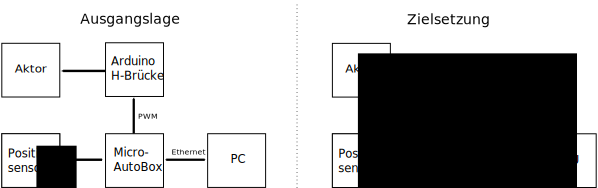
\includegraphics[width=0.9\columnwidth]{./Bilder/Ziel}%
\caption{Ausgangslage und Zielsetzung der Projektarbeit}%
\label{fig:Ziele}%
\end{figure} \indent
Auf der linken Seite sehen wir die Ausgangslage:  Die dSpace MicroAutoBox stellt dabei den Regler dar, der Istposition (bereitgestellt durch Positionssensordaten) und Sollposition (übermittelt über Ethernet vom PC) vergleicht und schließlich über pulsweitenmodulierte Spannungssignale eine H-Brücke ansteuert, welche wiederum den Aktor ansteuert. Dieser bewirkt die Bewegung der Schaltgabel und kann somit in verschiedene Gänge schalten. Auf der rechten Seite ist zu erkennen, wie das Gesamtsystem nach Abschluss der Projektarbeit optimalerweise aussehen sollte. Zentrales Element und Regler bildet hierbei die eingebettete Elektronik. Sie empfängt Daten vom Positionssensor, steuert den Aktor an und kommuniziert per CAN mit einem externen Steuergerät.

\section{Anforderungsliste}
Um das übergeordnete Ziel weiter zu spezifizieren wurde zunächst eine Anforderungsliste (\autoref{tab:Anforderungsliste}) erstellt. In dieser sind alle Forderungen an das Endprodukt gesammelt, sie dient damit als Basis und Referenz für die Produktentwicklung. Die Liste ist hierbei dynamisch, das heißt sie kann im Verlauf des Entwicklungsprozesses verändert oder ergänzt werden.  Die formulierten Anforderungen werden nach ihrer Priorität kategorisiert und einer der vier folgenden Anforderungsarten zugeordnet \cite[S.189]{2013a}. Festforderungen (FF) sind unter allen Umständen einzuhalten. Eine Erfüllung ist für eine erfolgreiche Lösung notwendig.
Bereichsforderungen (BF) geben einen Toleranzbereich an, innerhalb dessen sich der schlussendlich erreichte Wert befinden muss.
Zielforderungen (ZF) geben an, welcher Wert (auch im Hinsicht auf spätere Entwicklungen) angestrebt wird.
Wünsche (W) sollten nach Möglichkeit erfüllt werden, sind aber keine Voraussetzung. 

\begin{table}[h]
	\centering
		\captionabove{Anforderungsliste}
		\begin{tabular}{l|p{7cm}|p{7cm}}
			\textbf{Relevanz} & \textbf{Anforderung} & \textbf{Erläuterung} \\ \hline
			& &\\
			FF & Benutzerfreundliche Kommunikation durch CAN Schnittstelle & Empfang von Befehlen, Senden von Statusmeldungen \\ \hline
			FF & Nichtflüchtige Kalibrierung & Eine Kalibrierung ist nur einmalig und zur Rekalibrierung notwendig \\ \hline
			BF & Schaltzeit & < \SI{100}{ms} (Latenz zwischen Senden des Befehls und vollständig ausgeführtem Gangwechsel) \\ \hline
			FF & Selbstständige Fehlererkennung & Überstrom, Temperatur, Eingangsspannungsbereich, Dekalibrierung \\ \hline
			FF & Schnittstellen & CAN, \SI{8-16}{VDC} Versorgung, Programmierschnittstelle (für Updates \& Bugfixes) \\ \hline
			W & Wartbarkeit & Sicherung wechseln im eingebauten Zustand \\ \hline
			BF & kompakte Baugröße & 88,8x\SI{50}{mm}\\ \hline
			BF & Effizienz (gemittelt über einen Schaltvorgang) & elektrischer Wirkungsgrad > 90 \% \\ \hline
			FF & Temperaturbeständigkeit & bis \SI{105}{^\circ C} \\ \hline
			BF & Aktorüberschwingen & Toleriert, solange kein unbeabsichtigter Gangwechsel $\rightarrow$ \SI{<1}{mm} \\ \hline
			W & Schaltgabelkraft am Anschlag & möglichst gering \\ \hline
			FF & Standby & Standbyleistungsaufnahme < \SI{2}{W} \\ \hline
		\end{tabular}
	
	\label{tab:Anforderungsliste}
\end{table}

\section{Aufbau der Arbeit}
Nachdem in der Anforderungsliste nach \autoref{tab:Anforderungsliste} die Ziele der vorliegenden Arbeit definiert wurden, soll nun das weitere Vorgehen zum Erreichen der Zielsetzung erläutert werden. Zunächst werden in \autoref{kap2} der Stand des Prüfstands vor Beginn des Projektes sowie wichtige Grundlagen als Basis für die weitere Bearbeitung und zum besseren Verständnis dargelegt. \autoref{kap3} stellt das allgemeine methodische Vorgehen der Arbeit vor und erklärt die Entwicklungsmodelle und Testkonzepte, die angewendet wurden.
In \autoref{ch:komp} werden die verschiedenen Komponenten, die für die Elektronik benötigt werden, und ihre Funktionen beschrieben.  
In \autoref{kap5} soll schließlich der endgültige Platinenentwurf inklusive Methoden zur EMV-Verbesserung vorgestellt werden.
In Kapitel 6 wird nach der Vorstellung der entwickelten Software auch auf Optimierungsmöglichkeiten der Programmierung eingegangen.
Anschließend wird in \autoref{kap7} das Endprodukt auf seine Performance analysiert sowie die anfangs gestellten Anforderungen überprüft. Zum Abschluss wird in Kapitel 8 ein Fazit gezogen sowie ein Ausblick für weitere Forschungsarbeiten gegeben.
\chapter{Aufbau des Prüfstands und Grundlagen}
\section{Grundlagen des Prüfstandes}
In diesem Kapitel wird der verwendete Schaltaktorikprüfstand des IMS vorgestellt, an dem  die Entwicklung des Smart Actuators stattgefunden hat. Beschrieben wird der Aufbau des Prüfstands, wie er vor den Änderungen im Rahmen dieses Projektes vorlag. Die Konstruktion des Prüfstandes erfolgte in vorangegangenen Arbeiten und wurde seitdem stetig weiterentwickelt. An ihm werden Schaltaktoriksysteme für Fahrzeugantriebe untersucht. Abbildung \ref{fig:Pruefstand} zeigt die in dieser Arbeit verwendeten Subsysteme des Prüfstandes. Im Folgenden erfolgt zunächst die Vorstellung des mechanischen Aufbaus, woraufhin der elektronische Aufbau anschließt. 
\begin{figure}[h]
	\centering
		\includegraphics{Bilder/Pruefstand.jpg}
	\caption{Prüfstand \cite[S.5]{adp}}
	\label{fig:Pruefstand}
\end{figure}
\subsection{Getriebe allgemein}

Ein Getriebe ist im Automobil dafür zuständig, die Drehzahl des Motors in ein Drehmoment umzuwandeln, welches die Räder antreibt. Da Motoren nur einen kleinen Bereich von Motordrehzahlen abdecken werden mehrstufige Getriebe verwendet, die verschiedene Raddrehzahlen durch unterschiedliche Übersetzungsverhältnisse bereitstellen können.  Das Einstellen des jeweiligen Ganges kann dabei per Hand (Handschaltgetriebe) oder automatisiert über einen Aktor (Schaltaktorik) erfolgen. 
Im Fahrzeuggetriebe, beispielhaft dargestellt in \ref{fig:Fahrzeuggetriebe} ist die Eingangswelle, welche durch den Motor angetrieben wird, über eine Zahnradverbindung  fest mit der  Vorgelegewelle verbunden. Auf ihr sind noch weitere fest fixierte Zahnräder angebracht, deren Anzahl mit den verfügbaren Gängen übereinstimmt. Diese greifen jeweils in Losräder auf der Abtriebswelle. Um einen bestimmten Gang einzulegen muss nun das jeweilige Losrad für den Moment fest mit der Abtriebswelle verbunden werden, sodass nur diese Zahnverbindung ein Drehmoment überträgt. Dies geschieht über eine formschlüssige Verbindung mit einer Schaltmuffe, die über die durch den Aktor angetrieben Schaltgabel in Position gebracht wird.

\begin{figure}[h]
	\centering
		\includegraphics{Bilder/Fahrzeuggetriebe.jpg}
	\caption{Fahrzeuggetriebe}
	\label{fig:Fahrzeuggetriebe}
\end{figure}

\subsection{Getriebe des Prüfstands}

Der Prüfstand besitzt zwei Gänge, in die über eine Schaltgabel geschaltet werden kann. Eine Bewegung der Schaltgabel nach links legt Gang 1 über eine mechanische Synchronisierung ein, während mit Hilfe einer Bewegung nach rechts die Schaltung des Ganges 2 durch eine Klauenkupplung erfolgt. Somit können sowohl Schaltaktoriksysteme mit als auch ohne Synchronring untersucht werden.
Die Bewegung der Schaltgabel wird durch einen Linearaktor ermöglicht, welcher von außen an das Item-Profil verschraubt ist. In diesem ist eine Tauchspule verbaut, die die benötigten Kräfte auf die Läuferstange aufbringt. Über eine starre Wellenkupplung sind Läuferstange und Schaltgabel miteinander verbunden, wodurch die Kräfte auf die Schaltgabel übertragen werden und Schaltvorgänge ermöglicht werden.

\subsection{Aktor}

Der momentan in dem Prüfstand verbaute Tauchspulenaktor wurde von Oliver Hahn im Rahmen seiner Bachelorthesis entwickelt und konstruiert. Er übernimmt im automatisierten Schaltvorgang die Aufgabe, die Schaltgabel  über die Schaltstange translatorisch zu verschieben, welche ursprünglich mit einem Schalthebel per Hand ausgeführt wurde. Die Übertragung des Schaltbefehls an den Getriebeaktor erfolgt dabei durch ein elektrisches Signal (\textit{shift by wire})
Sein Querschnitt ist in folgender Abbildung schematisch dargestellt.

\begin{figure}[h]
	\centering
		\includegraphics{Bilder/Querschnitt Aktor.jpg}
	\caption{Querschnitt Tauchspulenaktor \cite[S.30]{Hahn2018}}
	\label{fig:Querschnitt Aktor}
\end{figure}

Sein Aufbau ist zylindrisch und kann in den ortsfesten Stator und den beweglichen Läufer unterteilt werden. Der Stator des Aktors besteht aus zwei in Reihe geschalteten Kupferspulen, welche fest in dem Gehäuse aus Weicheisen liegen und nach oben und unten mit Deckeln aus Aluminium fixiert werden. Der Läufer besteht aus einer nichtmagnetischen Läuferwelle, auf der sich fünf Permanentmagneten aus Neodym-Eisen-Bor befinden, welche mit Hilfe von zwei Polstücken aus Weicheisen axial auf der Läuferstange montiert sind. 
Werden nun die Kupferspulen von Strom durchflossen, so wirkt eine vom Magnetfeld der Permanentmagneten induzierte Lorentzkraft orthogonal auf sie. Diese Kraft ist abhängig von der Stromstärke I, der magnetischen Flussdichte der Permanentmagneten B und der vom Magnetfeld durchsetzten Leiterlänge l:
	\[F=I*l*B
\]
Da die Spulen jedoch fest im Gehäuse verbaut sind, wirkt eine entgegengerichtete Kraft auf die Permanentmagneten, die auf der axial verschiebbaren Läuferwelle lagern. Diese Kraft bewirkt dann eine translatorische Bewegung der Welle und somit auch der Schaltgabel. Die Richtung der translatorischen Bewegung kann dabei über die Richtung des in den Spulen fließenden Stromes, der Betrag der Kraft über den Betrag des Stromes eingestellt werden.
Anhand von Abbildung \ref{fig:Kennlinie Aktor} ist zu erkennen, dass die Kraft-Weg Kennlinien des Aktor innerhalb des Nutzungsbereichs von -10 Millimeter bis +10 Millimeter bei verschiedenen Stromstärken annähernd linear verlaufen. 

\begin{figure}[h]
	\centering
		\includegraphics{Bilder/Kennlinie Aktor.png}
	\caption{Kraft-Weg-Strom Kennlinien des Tauchspulenaktors \cite[S.12]{adp}}
	\label{fig:Kennlinie Aktor}
\end{figure}

\subsection{Aktoransteuerung}

Zur Aktoransteuerung wird ein Arduino IBT2 Motortreiber verwendet, die Stromversorgung erfolgt über ein Manson SBC-2130 Battery Charger im Power Supply Mode. Der Motortreiber besteht aus zwei BTS7960 MOSFETs, die je nach Vorgabe des pulsdauermodulierten Signals (PWM-Frequenz) eine Spannung von bis zu 13,8V an den Aktor durchschalten. 

\subsection{Autobox}


\subsection {Positionsmessung und -regelung}

Die Position der Läuferstange wird über einen PLCD-25M Sensor gemessen, dessen berührungslose PLCD (permanentmagnetic linear contactless displacement) Technologie die magnetische Sättigung nutzt. Der weichmagnetische Kern des Sensors ist über seine komplette Länge von einer Primärspule umgeben. Auf der Schaltgabel ist ein Permanentmagnet befestigt, welcher je nach Position zu einer lokalen Sättigung des weichmagnetischen Kerns führt. Über zwei Auswertungsspulen am Rand des Sensors kann nun die Position der Sättigungszone entlang der Sensorachse über eine induzierte Spannung bestimmt werden.

\begin{figure}[h]
	\centering
		\includegraphics{Bilder/Sensor.png}
	\caption{Einbauposition PLCD Sensor an der Schaltgabel \cite[S.14]{adp}}
	\label{fig:Sensor}
\end{figure}
Der Sensor wird an die MicroAutoBox zwecks Spannungsversorgung sowie zur Durchführung der Kalibrierung angeschlossen. Die Kalibrierung wurde in (Quelle) entwickelt und erfolgt bisher bei jedem Start. 

Die bisherige Regelung der Schaltgabelposition wurde in einem vorherigen Advanced Design Project ausgelegt. Dazu wurden mithilfe des Ziegler-Nichols-Verfahren zunächst Parameter für einen PID-Regler ermittelt, welcher allerdings noch zu große Totzeiten und ein Überschwingen aufwies. In einer anschließenden iterativen Optimierung mit Störgrößenkompensation wurden die Regelparameter zu KP =2,6\%V/mm, KI =20\%V/smm und KD =1,6\%Vs/mm bestimmt. Der Verlauf der Sprungantwort ist in nachstehender Abbildung (\ref{fig:Sprungantwort Schaltgabelposition}) dargestellt.
\begin{figure}[h]
	\centering
		\includegraphics{Bilder/Sprungantwort Schaltgabelposition.png}
	\caption{Sprungantwort Schaltgabelposition \cite[S.35]{adp}}
	\label{fig:Sprungantwort Schaltgabelposition}
\end{figure}

\section{Grundlagen Löten}
Löten gehört zu den Fügeverfahren und bezeichnet das Verbinden zweier Metalle durch eine Metalllegierung unter Einfluss von Wärme \cite{löten}. Die Metalllegierung wird dabei als Lot bezeichnet und hat eine geringere Schmelztemperatur (Liquidustemperatur) als die beiden zu verbindenden Metalle (Solidustemperatur). Durch das Löten entsteht eine feste, korrosionsbeständige sowie strom- und wärmeleitende Verbindung. Lötverfahren werden nach Arbeitstemperatur eingeteilt: es wird unterschieden in Weichlöten (bis 450°C), Hartlöten (450°C - 900°C) und Hochtemperaturlöten (über 900°C). Im Rahmen dieses Projektes wurde das Verfahren Weichlöten mit Lötkolben angewendet, um die elektrischen Bauteile auf der Platine anzubringen. Dazu konnten die vom Institut bereitgestellten Lötstationen und –materialien verwendet werden. 

\section{Mikrocontroller}
Ein Mikrocontroller (\textit{MCU: microcontroller unit}) ist ein hochintegrierter Halbleiterchip, der ein komplettes Mikrorechnersystem enthält. Prozessoren, Speicher, Ein- und Ausgabegeräte sind somit auf einem kleinen Chip enthalten der zum Ziel hat, Steuerungs- und Kommunikationsaufgaben möglichst simpel mit wenig Bauelementen zu bearbeiten. 
\begin{figure}[h]
	\centering
		\includegraphics{Bilder/Blockschaltbild Mikrocontroller.png}
	\caption{Blockschaltbild eines typischen Mikrocontrollers \cite[S.3]{Bernstein2015}}
	\label{fig:Blockschaltbild Mikrocontroller}
\end{figure}

In Abbildung \ref{fig:Blockschaltbild Mikrocontroller} ist der typische Aufbau eines Mikrocontroller dargestellt. Die Schnittstellen zur Peripherie sind durch einen Betriebsspannungsanschluss, einen Takteingang, an den in der Regel ein Quarz angeschlossen wird, sowie die Portleitungen  gegeben. Bei den Ports wird zwischen Eingangskanälen (\textit{\textbf{I}nput Port}), die digitale Signale lesen, und Ausgangskanälen (\textit{\textbf{O}utput Port}, die digitale Signale setzen beziehungsweise löschen, unterschieden. Des weiteren können I/O Pins digital oder analog sein, wobei analoge Signale mithilfe eines Analog/Digital Wandlers (AD-Wandler) zuerst in digital Signale umgewandelt werden müssen, damit der Mikrocontroller sie verarbeiten kann.
Eine Spezialform von Eingängskanälen sind die Interrupt-Pins, die bei bestimmten Ereignissen Unterbrechungen des laufenden Programms verursachen, um temporär einen anderen Vorgang zu bearbeiten. 

Intern sind die einzelnen Bausteine, die im folgenden kurz erläutert werden, über ein Bussystem verbunden.
Der Prozessor (\textit{CPU: central processing unit} führt Berechnungen und logische Operationen durch.
Der Taktgenerator gibt die Arbeitsfrequenz an, also wie schnell der CPU arbeiten soll.
Der Arbeitsspeicher (\textit{RAM: random access memory} speichert temporär Daten, die aber spätestens nach dem Entfernen der Betriebsspannung gelöscht werden.
Der Festspeicher (\textit{ROM: read only memory} behält seinen Speicherinhalt auch nach dem Entfernen der Betriebsspannung und enthält aufgrund dessen das Programm sowie Einstellungen und wichtige Daten. Im Vergleich zum RAM hat er eine langsame Schreibgeschwindigkeit. 
Der Timer hilft dabei, Anzahlen von Ereignissen zu zählen oder Zeitabstände zu messen, indem er Spannungswechsel an einem Eingangskanal zählt. 

Die genaue Ausführung des Chips kann je nach Aufgabentyp variieren, sodass eine Vielzahl an verschiedenen Mikrocontrollern erhältlich ist. Diese unterscheiden sich meistens in der Größe des Speichers, in der Anzahl der Anschlüsse beziehungsweise Schnittstellen, in der Bitbreite, in den Taktraten sowie in der Bauform. Typischerweise werden Mikrocontroller in eingebetteten Systemen (\textit{embedded systems} verwendet, bei denen die Steuereinheit direkt im System selbst integriert ist. Übliche Anwendungen für Mikrocontroller sind Roboter, Handys, Temperaturregler oder Motorsteuerungen \cite{Brinkschulte}. 




\section{Eingebettete Systeme und Smart Actuators}
Eingebettete Systeme werden definiert als Rechenmaschinen, die für den Anwender weitgehend unsichtbar in einem technischen System eingebettet sind und mit diesem in Wechselwirkung stehen \cite[S.8]{Gessler2014}. Der Rechner kann dabei für Regelungs-, Steuer- oder Überwachungsaufgaben und/ oder für Signal- und Datenverarbeitung zuständig sein. Der allgemeine Zweck ist es, die Stellglieder als Reaktion auf Eingangssignale, die von Sensoren oder manuell vorgegeben werden, zu steuern \cite[S.1]{Broy2003}. Eingebettete Systeme werden oft für speziell eine isolierte Aufgabe entwickelt und angepasst.
Ein Aktor, beziehungsweise Aktuator (aus dem englischen: \textit{actuator}) ist dafür da, die elektrischen Signale in eine Bewegung oder Kraft umzusetzen und bildet somit das Stellglied. 
Ein intelligenter Aktor (\textit{smart actuator}) ist definiert als das integrierte Stellglied inklusive aller Komponenten wie Motor, Steuerung, Sensorik und Kommunikationseinheit \cite[S.442]{smartactuator}.
Das Konzept besteht darin, den Aktor um Informationsverarbeitungs- und Kommunikationsmöglichkeiten zu erweitern, der Aktor enthält dann die eingebettete Elektronik.
Smart Actuators reduzieren beziehungsweise ersetzen die benötigte Interaktion mit einem Menschen oder externen Rechner und können somit effektiver und schneller arbeiten. Außerdem kann oft viel Bauraum eingespart werden, es gibt weniger Komponenten und deutlich weniger Verkabelung, womit der Einbau in ein Gesamtsystem leichter ist. Hervorzuheben sind weiterhin die verringerten Kosten, die Überwachung und Diagnose des eigenen Zustands sowie die verbesserte Präzision. Einbußen müssen Smart Actuators allerdings in Sachen Flexibilität, da sie oft für eine spezielle Aufgabe ausgelegt sind und ihr Verhalten stark vorgegeben ist \cite[S.4]{smartaktor}.


\section{Controller Area Network (CAN)}
Um eine Kommunikation zwischen zwei Geräten (z.B. Sensoren, Aktoren und Steuergeräten) zu ermöglichen, muss ein System zur Datenübertragung vorhanden sein. Dabei hat sich bei vielen PKW- und NKW-Herstellern  das Controller Area Network (CAN) durchgesetzt \cite[S.15]{} CAN ist ein von Bosch für den Automobilbau entwickeltes Bussystem, mit dem mehrere gleichberechtigte Teilnehmer verbunden werden und miteinander kommunizieren können \cite[S. 278]{}.
Für ein CAN-Netzwerk werden zwei Leitungen CAN-High und CAN-Low benötigt, an denen alle zu verbindenden Teilnehmer parallel angeschlossen sind. Die beiden Leitungen werden an beiden Enden mit Wellenwiderständen von 120 Ohm verbunden. Der schematische Aufbau eines CAN-Buses mit zwei Teilnehmern ist in Abbildung \ref{fig:CAN} dargestellt. 

\begin{figure}[h]
	\centering
		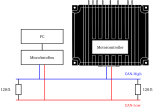
\includegraphics{Bilder/CAN.pdf}
	\caption{Aufbau CAN-Bus}
	\label{fig:CAN}
\end{figure}


Sollten mehrere Teilnehmer gleichzeitig versuchen eine Nachricht zu senden und somit ein gleichzeitiger Buszugriff vorliegt, kommt es zu einer Kollision. Um diese Aufzulösen wird ein CSMA/CR-Verfahren (\textit{Carrier Sense Multiple Access/Collision Resolution}) verwendet, bei dem die höher gewichtete (dominante) Nachricht die niedriger gewichtete (rezessive) Nachricht überschreibt, sodass der Übertragungsversuch beendet wird. Die Einteilung der Relevanz einer Nachricht erfolgt auf Basis der sogenannten Identifier(ID)-Bits, wobei niedrige ID-Bits eine höhere Relevanz als höhere ID-Bits haben. Dadurch wird eine Hierarchie der Nachrichten erzeugt, wodurch die Nachricht mit der niedrigsten ID immer gesendet werden darf. Dementsprechend werden wichtigen Nachrichten niedrige IDs zugeteilt (QUELLE). 
Die Geschwindigkeit der Datenübertragung zwischen den Teilnehmer ist dabei von der Länge der Leitungen abhängig und beträgt maximal 1Mbit/s. Nach [ZS14, S. 58] kann die Bitrate überschlagsmäßig mit 
\begin{equation}
	Buslaenge<40...50+++++++
	\label{eq:CAN}
\end{equation}

berechnet werden.

Im Folgenden wird speziell auf die in dieser Arbeit eingerichtete CAN-Kommunikation und den Aufbau der CAN-Nachrichten eingegangen: Es wird ein CAN-Bus verwendet, mit dem lediglich zwei Teilnehmer miteinander verbunden werden. Diese sind zum einen die MicroAutoBox und zum anderen der Mikrocontroller des Smart Actuators. Die Länge der Leitungen zwischen den beiden ist wesentlich kürzer als 3m, wodurch nach Formel (\ref{eq:CAN}) die maximale Bitrate von 1Mbit/s genutzt wird.

\chapter{Vorgehensweise und Testverfahren}\label{kap3}
Das folgende Kapitel thematisiert, wie während des Projekts vorgegangen wird, welche Entwicklungsmodelle zum Einsatz kommen und welche Testkonzepte angewendet werden.

\section{Entwicklungsmodell}
Sowohl für die Entwicklung eines Softwaresystems als auch für die Entwicklung von Elektronik haben sich Modelle etabliert, die eine Systematik in den Entwicklungsprozess bringen. Dadurch soll eine hohe Qualität des Entwicklungsprodukts sichergestellt werden. 
Unter Qualität, insbesondere bei Softwaresystemen, werden nach \cite{BasSof} bzw. ISO-Norm 25010 \cite{ISO_25010} Eigenschaften verstanden wie Funktionalität, Zuverlässigkeit, Benutzbarkeit, Effizienz und Änderbarkeit.

Für die vorliegende Aufgabenstellung ist ein Softwaresystem zur
\begin{itemize}
	\item Verarbeitung der Sensorik,
	\item Anwendung des Regelgesetzes,
	\item Ansteuerung der Aktorik,
	\item nichtflüchtige Kalibrierung und
	\item selbstständige Fehlererkennung
\end{itemize}
notwendig. Gleichermaßen muss jedoch eine Elektronik entwickelt werden, auf welcher das Softwaresystem ausgeführt wird und durch welche die Schnittstelle zu notwendigen Komponenten hergestellt wird. Um beide Systeme parallel zu entwickeln wird das V-Modell gewählt, das in \autoref{fig_v_modell} dargestellt ist. 



\subsection{Das V-Modell}

\begin{figure}%
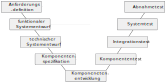
\includegraphics[width=\columnwidth]{./Bilder/fig_v_modell}%
\caption{V-Modell nach \cite{Boehm79}}%
\label{fig_v_modell}%
\end{figure}

Das V-Modell ist ein Vorgehensmodell, dass in verschiedenen Ausführungen existiert. Das hier vorgestellte und angewendete Modell entspricht dem Modell nach \cite{Boehm79}. Als weitere Quelle wird \cite{BasSof} herangezogen und im Folgenden referenziert.
Der linke Zweig stellt dabei die konstruktive Entwicklung dar, während jede Aktivität eine dazu korrespondierende Testaktivität im rechten Zweig besitzt. \\

\subsubsection{Konstruktive Entwicklung (linker Zweig)}
Zunächst wird demnach eine Anforderungsliste im Zuge der \textit{Anforderungsdefinition} erstellt, die die Entwicklungsaufgabe genauer spezifiziert und später eine Überprüfungsgrundlage bietet inwiefern das fertige Gesamtsystem des Wunschsystems entspricht. Daran anschließend wird ein \textit{funktionaler Systementwurf} durchgeführt. Hierbei werden die Anforderungen in Funktionen überführt, die das Gesamtsystem erfüllen muss, um den Anforderungen gerecht zu werden. Darauf folgend findet der \textit{technische Systementwurf} statt. Dafür wird das System in unabhängige Teilsysteme unterteilt und Schnittstellen zur Umwelt ermittelt. Daran logisch anknüpfend wird die \textit{Komponentenspezifikation} durchgeführt. Dafür wird für jede Komponente (elementares Teilsystem) die Aufgabe, das gewünschte Verhalten und Schnittstellen zu anderen Teilsystemen definiert. \\
Den letzten reinen Entwicklungsschritt bildet die \textit{Komponentenentwicklung}. Dabei werden schließlich die einzelnen Komponenten nach der zuvor erarbeiten Spezifikation entwickelt. Eine Komponente stellt dabei ein Teilsystem dar, das eine feste Funktion erfüllt, und in der Regel aus einem Softwareteil und einem Hardwareteil besteht. Beide Teile werden parallel in genauer Abstimmung entwickelt, da die gewünschte Funktion nur durch beide Systeme im Zusammenspiel erfüllt werden kann. Das Softwaresystem besteht dabei in der Regel aus einem Treiber, der die komplexe Hardwareschnittstelle für das Restsystem versteckt und komfortable Schnittstellen bereitstellt. Ein Beispiel dafür stellt der Treiber für den Tauchspulenaktor dar, der eine Pulsweite in Prozent und ein Aktivierungssignal entgegen nimmt. Intern werden dann daraus Steuersignale für die Halbbrücken generiert und über die Elektronikschaltung dem Aktor zugeführt.
Neben Elektronikschaltungen mit zugehörigem Treiber existieren auch \textit{reine Softwarekomponenten}, die unabhängig der Elektronik entwickelt werden wie bspw. eine Verhaltenslogik für ein- und ausgehende CAN-Nachrichten. Ebenso existieren \textit{reine Elektronikkomponenten}, die keinen direkten Bezug zur Software aufweisen und daher unabhängig zur Software entwickelt werden können.\\

\subsubsection{Testaktivitäten (rechter Zweig)}
Alle folgenden Informationen sowie detaillierte Ausführungen bezüglich des Testverfahrens können \cite{BasSof} entnommen werden.\\
Nachdem die Entwicklung aller Komponenten abgeschlossen ist, müssen die einzelnen Komponenten auf die geforderte Funktionalität überprüft werden. Dazu wird jede Komponente so isoliert wie möglich vom Restsystem getestet, ggf. unter Einsatz sogenannter Testtreiber und Platzhalter, um die zu testenden Komponenten mit Testdaten oder Testfällen auszuführen. Durch die Isolation wird sichergestellt, dass die einzelne Komponente als solche funktioniert und Fehlerzustände leichter eingegrenzt und lokalisiert werden können. Jeder Testfall enthält dabei feste Vorbedingungen, Eingabewerte und ein gefordertes Sollverhalten bzw. geforderte Ausgabewerte. Die Auswahl der Testfälle wird durch die Art der Komponenten unterschieden. \textit{Treiber mit zugehöriger Hardwarekomponente} bieten Schnittstellen, die beliebige Zahlenwerte und Kombinationen entgegen nehmen. Daraus resultiert eine quasi unendliche Menge an möglichen Testfällen, die nicht praktikabel getestet werden können. Vollständiges Testen ist daher nicht möglich. Aus diesem Grund werden die Testfälle aus einem Klassifikationsbaum mit anschließender Grenzwertanalyse gewonnen. Dabei wird jeweils mindestens ein Testwert aus jeder Gruppe ausgewählt. Die Gruppierung wird so vorgenommen, dass von jeder Gruppe aus Testwerten gleiches Verhalten angenommen wird. Als Beispiel kann wieder die Ansteuerung des Tauchspulenaktors herangezogen werden. Es wird davon ausgegangen, dass alle Werte zwischen -100 und 0 eine Bewegung in eine feste Richtung bewirken. Dagegen bewirken Werte von 0 bis 100 eine Bewegung in die Gegenrichtung. Werte außerhalb des Zahlenbereichs werden auf entsprechend -100 oder +100 abgerundet. Durch eine Grenzwertanalyse werden diese Gruppen (auch Äquivalenzklassen genannt) noch in Untergruppen unterteilt, in denen die oft kritischen Grenzwerte (-100, 0 und 100) noch eigene Gruppen bilden. Eine Sonderstellung besitzt die Null, weil hier keine Reaktion erwartet wird. Durch kombinatorische Paarbildungen werden darüber hinaus auch beliebige Kombinationen aus abhängigen Eingangswerten, bspw. Aktivierungssignal (enable) und Pulsbreite (PWM [\%]), berücksichtigt. Um die Testfallgenerierung durch Klassifikationsbäume zu verdeutlichen, ist in \autoref{fig_klass} der Klassifikatiosbaum grafisch dargestellt. Die untere Zeile aus konkreten Werten stellt beispielhafte Testwerte aus der darüberliegenden Äquivalenzklasse dar. Darunter ist über die Gitterstruktur angedeutet wie aus der paarweisen Kombination der einzelnen Testwerte Testfälle bestimmt werden. \textit{Testfall 1} entspricht dem Aufrufen des Treibers mit einer PWM von \SI{-100}{\%} und einem aktivierten \textit{enable}-Signal. Es wird daher erwartet, dass der Aktor voll in \glqq negative\grqq{} Bewegungsrichtung bestromt bzw. beschleunigt wird. Ob die Elektronik als solche den Erwartungen bzw. der Spezifikation entspricht, kann durch Strom-/Spannungs- sowie Temperaturmessungen verifiziert werden. 
\begin{figure}%

\includegraphics[width=\columnwidth]{./Bilder/fig_klass}%
\caption{Klassifikationsbaum am Beispiel des Motortreibers}%
\label{fig_klass}%
\end{figure}
\\
Für \textit{reine Softwarekomponenten} hingegen werden Testfälle auf eine geeignetere Weise generiert. Bei Softwarekomponenten auf Basis eines Zustandsautomaten werden Testfälle aus einer zustandsbasierten Testfallgenerierung gewonnen. Dabei wird als Testziel vorausgesetzt, dass alle Entscheidungen (Kanten) eines Zustandsautomaten mindestens einmal ausgeführt werden, was als Entscheidungsüberdeckungskriterium bezeichnet wird. Dieses Kriterium schließt auch automatisch ein, dass alle Zustände (Knoten) besucht worden sind. Wie viele Testfälle getestet werden müssen hängt dabei stark von der Größe und Komplexität des Zustandsautomaten ab.\\
Nach dem Test der einzelnen Komponenten wird eine Integration vollzogen. Unter Integration versteht man dabei das Zusammenführen der Komponenten zu einem Gesamtsystem. Es stehen viele Varianten zur Verfügung, dazu zählen \textit{Bottom Up}-, \textit{Top Down}- und \textit{Big Bang}-Integration. Letztere Variante sieht vor, dass alle Komponenten in einem Zug ins Gesamtsystem integriert werden. Auftretende Fehler können jedoch in diesem Fall nur schwierig zugeordnet werden. Günstiger ist daher die \textit{Bottom Up}-Integration, wobei nach und nach Komponenten hinzugefügt werden und übergeordnete Komponenten, die mit mehreren Einzelkomponenten Schnittstellen haben, später integriert werden. Da im vorangehenden \textit{Komponententest} bereits die Komponenten getestet sind, ist im anschließenden \textit{Integrationstest} mit Fehlern zu rechnen, die durch Schnittstellen zwischen den Komponenten hervorgerufen werden. Es kann davon ausgegangen werden, dass die Komponenten intern funktionieren und ausschließlich das Zusammenspiel der Komponenten fehlerhaft ist. \\
Zuletzt entsteht somit ein Gesamtsystem, das darauf getestet werden muss, ob die im \textit{funktionalen Systementwurf} festgelegten Funktionen erfüllt werden. Um dies zu testen werden \textit{Use-Case}-Szenarios erstellt, die eine übliche Nutzung simulieren. Dabei wird von mehreren Akteuren ausgegangen, die mit dem System in der realen Anwendung agieren werden. Der Schaltaktor wird bspw. über ein übergeordnetes Steuergerät (\textit{electrical Control Unit}) angesteuert. Die Schnittstelle wird durch CAN realisiert, sodass ein entsprechendes Steuergerät über CAN Signale/Befehle einen Schaltvorgang anfordern kann oder eine Fehlermeldung auslesen kann. Einen typischen \textit{Use-Case} würde bspw. ein Schaltbefehl vom neutralen in den zweiten Gang darstellen. Dieser kann erfolgreich ablaufen oder durch eine mechanische Blockade verhindert werden. Abschließend erfolgt der Abnahmetest, der in der Regel durch den Auftraggeber durchgeführt wird. Hier wird explizit verglichen, ob die versprochenen Leistungen im Pflichtenheft auch erreicht werden.

Diese und weitere Informationen für den interessierten Leser finden sich in \cite{BasSof}.

\subsection{Konkretes Vorgehen mit inkrementellem Entwicklungsansatz}

Neben dem V-Modell fließen auch inkrementelle Ansätze in die Entwicklung ein. So wird das V-Modell mehrmals durchlaufen, während nach jeder Iteration ein ausführbares und testbares Entwicklungsprodukt vorliegt. Diese Zwischenprodukte entsprechen der Anforderungsliste unter Umständen nur teilweise, sodass mehrere Iterationen bis zu einem zufriedenstellenden Produkt notwendig sind. Für das vorliegende Projekt wird in der ersten Iteration ein Prototyp angestrebt, der bereits die Grundfunktionalitäten bereitstellt. Dies umfasst die Möglichkeit, einen Schaltvorgang nach Anforderungsspezifikation durchzuführen. Dafür muss unter Anderem die Aktorik ansteuerbar sein und die Sensorik notwendige und hinreichend genaue Regelgrößen liefern. 
Während der Phase des Prototyping wurde der Mikrocontroller auf einem Entwicklungsboard verwendet, um Daten über die USB-Schnittstelle mit dem PC austauschen zu können, über die der Mikrocontroller auch programmierbar ist, und alle Pins leicht über Stiftleisten erreicht werden können. Die Funktionalität der geplanten Brückenschaltung zur Aktorsteuerung wurde dafür zunächst unabhängig vom Aktor getestet, um seine Sicherheit zu gewährleisten. Dies wurde der Einfachheit halber auf Steckbrettbasis und mit Anschluss zweier LEDs statt dem Motor durchgeführt. Die PWM-Frequenz konnte dabei die Helligkeit der LEDs steuern und durch verschiedene Eingangssignale in die schaltenden Transistoren wurde vorgegeben, welche der beiden LEDs leuchten soll. Um für den ersten Prototypen mit dieser Schaltung den Aktor anzusteuern, wurde der Leistungsteil mit THT-Bauteilen (\textit{through hole technology}-Bauteilen) auf eine Lochrasterplatine gelötet, da durch ihn größere Ströme als für Steckbrett empfohlene 1 Ampere fließen.
Die Elektronik für den Lagesensor, welcher bereits von Vorgängerprojekten genutzt wurde, wird ebenfalls auf einem Steckbrett realisiert. Um den Prototypen schließlich in Aktion zu testen, wird ein Testprogramm geschrieben und auf den Mikrocontroller geflasht. Anforderungen an Größe, Effizienz oder Integrierbarkeit sind bei diesem ersten Prototypen nicht verfolgt worden. Durch das Ergebnis werden Erkenntnisse gewonnen, die in den nächsten Iterationen berücksichtigt werden. 
Bei folgenden Iteration wird versucht über geeignete Maßnahmen (bspw. durch eine angepasste Komponentenspezifikation) bisherige Ergebnisse zu verbessern und weitere Anforderungen zu erfüllen. 
Hierfür rückt besonders die iterative Weiterentwicklung der Software in den Vordergrund, da fast die komplette benötigte Hardware zur Anforderungserfüllung bereits im ersten Prototypen Anwendung findet. %Nichtflüchtige Kalibrierung/ CAN etc%
Im nächsten Schritt wurde an der automatischen Fehlererkennung gearbeitet. Um Strommesswerte zu erhalten wurde, musste die integrierte Strommessung der verwendeten Halbbrücken über den Statuspin vom Mikrocontroller ausgelesen werden. Zur Erkennung von Übertemperatur im Aktor wird ein externer Temperatursensor angeschlossen und ausgelesen.
Einen wesentlichen Iterationsschritt stellt schließlich der Übergang von Steckbrett- auf Platinenbasis dar. Durch diesen Übergang treten weitere Anforderungen wie Baugröße und Integrierbarkeit in den Vordergrund. Nach dem letzten Iterationsschritt sollten alle Anforderungen nachweislich erfüllt sein, sodass ein erfolgreicher System- und Abnahmetest durchgeführt werden kann. In \autoref{fig_entw_evo} sind die Iterationen exemplarisch dargestellt, während in \autoref{tab_entw_evo} ein beispielhafter Ausschnitt aus dem Ergebnis des jeweiligen \textit{Systemtests} pro Iteration dargestellt sind.

\begin{table}%
\centering
\captionabove{Beispielhafter Ausschnitt aus Systemtest-Ergebnissen über mehrere Iterationen}
\begin{tabular}{c c c c c c c}
Iteration & Schaltzeit & Nichtflüchtige Kalibrierung & kompakte Baugröße & Effizienz & Fehlererkennung & ...  \\
\hline
1 & \checkmark  & \checkmark & \texttimes & \texttimes & \texttimes & ...  \\
2 & \checkmark & \checkmark & \texttimes & \texttimes & \checkmark  & ...   \\
3 & \checkmark & \checkmark & \texttimes & \checkmark & \checkmark  & ...   \\
...    \\
\end{tabular}
\label{tab_entw_evo}
\end{table}

\begin{figure}%
\centering
\includegraphics[width=0.7\columnwidth]{./Bilder/fig_entw_evo}%
\caption{Bildliche Darstellung des Prototypings (Iterationsprozesses)}%
\label{fig_entw_evo}%
\end{figure}

\chapter{Auswahl elektronischer Komponenten und Verschaltung}\label{ch:komp}
Im Folgenden wird auf die Auswahl der Platinenkomponenten, sowie deren Beschaltung eingegangen. Der gesamte Schaltplan ist in \autoref{app:boardlayout} angefügt.
\section{Anforderungen an die Komponenten}
Elektronische Komponenten sind üblicherweise in passive und aktive Bauelemente untergliedert. Unter passiven Bauelementen werden Komponenten verstanden, die das Eingangssignal ohne Verstärkung übertragen. Aktive Bauelemente benötigen meist eine Hilfsquelle und können somit ein Eingangssignal verstärken \cite[S.25]{haendschke}. Für den Einsatz elektronischer Komponenten im Automobilbereich hat sich für passive Bauteile die Zertifizierung nach AEC-Q200 und für aktive Bauteile nach AEC-Q100 als Qualitätsstandard etabliert. Anhand dieser Zertifizierungen wird eine nachweisliche Belastbarkeit der Bauelemente nach dem jeweiligen Standard definiert. Für die Anforderungen an die Platine werden die passiven Bauelemente nach AEC-Q200 und die aktiven Bauelemente nach AEC-Q100 mindestens in \textit{Grade 2} eingestuft, um den Temperaturanforderung bis \SI{105}{^\circ C} gerecht zu werden \cite[S.6]{aecq}. 
\subsection{Passive Bauteile}
Unter die benötigten passiven Bauteile fallen Kondensatoren und Widerstände, welche nach dem AEC-Q200 Standard ausgewählt werden. Anforderung ist danach eine thermische Belastbarkeit von mindestens \SI{105}{^\circ C}. Um eine geringe Baugröße der Platine zu gewährleisten, sollten sowohl Widerstände als auch Kondensatoren als SMD-Bauteil (\textit{surface-mounted device}) gewählt werden. Für Abblockkondensatoren werden nach \cite[S.7]{ldo} Keramikkondensatoren mit XR7 präferiert. Diese werden einerseits dazu genutzt, um bei impulsartiger Netzbelastung durch hohe Leistungsaufnahme von ICs das Netz zu entlasten, andererseits aber auch um Restwelligkeiten zu filtern. Als Baugröße bei manueller Bestückung bieten sich die Standardgrößen 1206 oder 0805 (Angabe in $\frac{1}{100}$ Zoll), welche noch per Hand lötbar sind. Die Widerstände für die Sensorik müssen mit sehr hoher Präzision, geringem Rauschen und niedriger Temperaturabhängigkeit gewählt werden, um Messfehler aufgrund falscher Widerstandswerte zu vermeiden. Im Anwendungsfall bieten sich daher Dünnschichtwiderstände an.
\subsection{Aktive Bauteile}
Die aktiven Bauelemente der Platine müssen dafür ausgelegt werden, um im Späteren alle Anforderungen aus der Anforderungsliste (vgl. \autoref{tab:Anforderungsliste}) gerecht zu werden. Demnach müssen sie in ihrer logischen Verschaltung einerseits in der Lage sein den Tauchspulenaktor anzusteuern und auszuregeln, andererseits aber auch die Bedingungen über Leistungsaufnahme etc. erfüllen. Kern der Platine ist ein Mikrocontroller, welcher schnell genug sein muss, um Gangwechsel in weniger als \SI{0,1}{s} durchzuführen. Weiterhin muss der Mikrocontroller die CAN-Kommunikation mit der MicroAutobox unterstützen. Da der Mikrocontroller nicht über die \SI{13,8}{V} der Autobatterie gespeist werden kann, wird ein Spannungsregler benötigt, welcher auf die Betriebsspannung des Mikrocontrollers regelt. Um aus den physikalischen Bussignalen CAN-HIGH und CAN-LOW für den Mikrocontroller verwertbare Signale zu erhalten wird ein CAN-Transciever benötigt. Über diesen ist eine Kommunikation des Mikrocontrollers mit der CAN-Peripherie erst möglich. Zum Regeln des Tauchspulenaktors ist ein Motortreiber nötig, welcher vom Mikrocontroller angesteuert wird, um die Spannung an den Tauchspulenaktor durchzuschalten. Eine Ansteuerung des Motortreibers mittels PWM-Signal sollte möglich sein. Der Motortreiber muss dabei für zukünftige Aktorkonfigurationen für Ströme bis zu \SI{55}{A} ausgelegt sein. Des Weiteren wird eine Spannungsebene von \SI{5}{V} benötigt um die Lagesensorik des Aktors zu unterstützen, wofür ein zweiter Spannungsregler eingeplant werden muss.
%\begin{figure}[H]%
%\centering
%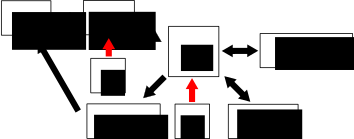
\includegraphics[width=250pt]{./Bilder/anf.pdf}%
%\caption{Benötigte Ebenen der Verschaltung}%
%\label{fig:anf}%
%\end{figure}
\newpage
\section{Komponentenauswahl}
Anhand der Anforderungen an die Platinenelemente sind die endgültigen Komponenten der Platine zu wählen. Es müssen Mikrocontroller, Spannungsregler, CAN-Transciever und Motortreiber ausgewählt werden. Weiterhin wird eine Temperaturbeständigkeit bis \SI{105}{^\circ C} gefordert.
\subsection{Mikrocontroller}\label{sec:mcu_kap4}
Die Recheneinheit zur Regelung des Tauchspulenaktors ist ein STM32F405RGT7-Mikrocontroller. Dieser ist mit verschiedenen Pin-Anzahlen erhältlich und auf der Platine aus Platzgründen in der Ausführung LQFP64 mit 64 Pins verbaut. Der Mikrocontroller zeichnet sich durch seine hohe CPU-Geschwindigkeit von \SI{168}{MHz} und seine große Programm-Speichergröße von \SI{1}{MB} aus. Die Namensendung -T7 steht dabei für die zulässige Betriebstemperatur von -40...\SI{105}{^\circ C}. Weiterhin besitzt dieser Mikrocontroller die geforderten CAN-Schnittstellen, anhand derer mit der MicroAutobox kommuniziert werden soll. In \autoref{fig:mcumin} ist die Minimalbeschaltung des Mikrocontrollers zu sehen. Diese ist dem Datenblatt des STM32 entnommen \cite[S.77]{stm32} (vgl. \autoref{app:stm32man}). Die Pins mit den Bezeichnungen VDD bis VDD\_4 sind die Versorgungspins des Mikrocontrollers. An diesen Pins liegt die Versorgungsspannung an, welche nach dem Datenblatt zwischen 1,8 und \SI{3,6}{V} liegt. Diese ist aufgrund der Versorgungsspannung anderer Bauteile zu VDD = \SI{3,3}{V} gewählt. Die VDD Pins werden durch die Keramikkondensatoren C7 bis C11 entkoppelt, welche nach dem Datenblatt dimensioniert sind und möglichst nah an den dem jeweiligen VDD-Pin plaziert werden sollen. Die Entkopplung wird benötigt, um Welligkeiten der Spannungsversorgung zu filtern und parasitäre Induktivitäten zu entkoppeln \cite{decoupling}. Der Pin VBAT wird unter Anderem für die Versorgung der Echtzeituhr (\textit{RTC}), der Backup-Register und des Backup-SRAMs genutzt und wird, wenn keine zweite Spannungsversorgung neben der Hauptversorgung vorhanden ist, ebenfalls an VDD angeschlossen \cite[S.31]{stm32}. VDDA ist der Pin für die Spannungsversorgung des Analog-Digital-Converters (\textit{ADC}) und wird ebenfalls mit der Versorgungsspannung von VDD angeschlossen. Die Kapazitäten C5 und C6 sind nach den Herstellerangaben dimensioniert und sorgen ebenfalls für eine Entkopplung der Spannungsversorgung. Die Induktivität L1 bietet die Möglichkeit, je nach Welligkeit der Versorgungsspannung, diese über einen LC-Filter zu filtern um eine bessere Auflösung des ADCs zu gewährleisten. Wenn dieser Filter nicht benötigt wird, sollte L1 durch einen \SI{0}{\Omega} Widerstand ersetzt werden.
VCAP\_1 und VCAP\_2 sind die Ausgänge des internen Voltage Regulators des STM32 und C5 bzw. C6 werden zur Glättung der intern geregelten Spannung genutzt \cite[S.77]{stm32}. Die Pins VSS, VSS\_2 und VSSA sind die GND Anschlüsse für den Mikrocontroller und den internen ADC.
\begin{figure}[H]%
\centering
\includegraphics[width=\columnwidth]{./Bilder/MCU_MIN.pdf}%
\caption{Minimalbeschaltung des STM32F405RGT7}%
\label{fig:mcumin}%
\end{figure}\noindent
In \autoref{fig:mcupin} sind die Pin-Belegungen des Mikrocontrollers dargestellt, welche durch \autoref{tab:pins} genauer beschrieben sind. Unter Sensorik fallen die Ausgänge für Lagesensorik, Temperatursensorik und Messung der Versorgungsspannung. Die UART Pins können zum \textit{debuggen} auf der endgültigen Platine genutzt werden. Zur CAN-Kommunikation werden die Pins CAN1-TX (PA11) und CAN1-RX (PA12) benötigt, womit der Mikrocontroller über einen CAN-Transciever Nachrichten an die MicroAutobox senden und ebenfalls Nachrichten von dieser empfangen kann. Zum Programmieren des Mikrocontrollers wird eine \textit{SWD}-Schnittstelle aufgebaut, welche sich mittels externem ST-Link/V2 mit dem Computer verbinden lässt. Dazu werden die jeweiligen Pins über den Platinenstecker nach außen geführt (vgl. \autoref{fig:stecker}). Weiterhin müssen Pins zum Beschalten der H-Brücke und zum Auslesen der Strommessungen belegt werden. Die Pins OSC\_IN und OSC\_OUT sind zum Anschließen eines externen Quarzes, welcher als Taktgeber für den Mikrocontroller genutzt wird. Der Pin NRST wird für den Fall eines notwendigen Resets herausgeführt. Über diesen kann der Mikrocontroller bei Fehlern im Befehlszähler (\textit{program counter corruption}) wieder in den Initialzustand des Programms zurückgesetzt werden. Daten aus dem Flash-Speicher bleiben dabei unverändert. Dazu muss der NRST-Pin für eine Sekunde extern auf \textit{low} (0 bis \SI{0,8}{V}) gezwungen werden \cite[S. 111]{stm32}. Somit ist im Falle eines undefinierten Programmzustands auch im eingebauten System ein Programmneustart ohne Datenverlust möglich.

\noindent\begin{minipage}{0.75\textwidth}
\includegraphics[width=\textwidth]{./Bilder/MCU_PINS.pdf}
\end{minipage}
\noindent\begin{minipage}{0.1\textwidth}
\begin{tabular}{l | l}
			Pin & Funktion\\ \hline
			PA0& Sensorik\\
			PA1& Sensorik\\
			PB0& Sensorik\\
			PB1& Sensorik\\
			PC2& Sensorik\\
			PC3& Sensorik\\
			PC5& Sensorik\\
			PA2& UART\\
			PA3& UART\\
			PA11& CAN\\
			PA12& CAN\\
			PA13&SWD\\
			PA14&SWD\\
			PB3& SWD\\
			PB0 & H-Brücke\\
			PB1 &H-Brücke\\
			PB10&H-Brücke\\
			PB11&H-Brücke\\
			PC4&H-Brücke\\
			OSC\_IN&Quarz\\
			OSC\_OUT&Quarz\\
			NRST & Reset
		\end{tabular}
\end{minipage}

\noindent\begin{minipage}{0.75\textwidth}
\captionof{figure}{Pin-Belegung des Mikrocontrollers}
\label{fig:mcupin}
\end{minipage}
\noindent\begin{minipage}{0.2\textwidth}
	\captionof{table}{Pin-outs}
	\label{tab:pins}
\end{minipage}
\hspace{1cm}
\newline
\\
Wichtig bei der Beschaltung ist außerdem die Belegung von BOOT0 und BOOT1, welche den Speicherbereich definieren aus dem der Mikrocontroller beim Startvorgang sein Programm lädt. Nach \autoref{tab:boot} muss für den Start im Main Flash memory BOOT0 auf GND-Niveau gesetzt werden, während die Belegung von BOOT1 undefiniert ist und somit mit GND belegt werden kann.

\begin{table}[H]%
\centering
\captionabove{Boot modes des STM32F405RGT7 nach \cite[S.69]{stmref}}
\begin{tabular}{c c c c}
BOOT1 & BOOT0 & Boot mode & Aliasing \\ \hline
x & 0 & Main Flash memory & Main Flash memory is selected as the boot space\\
0 & 1 & System memory & System memory is selected as the boot space\\
1 & 1 & Embedded SRAM & Embedded SRAM is selected as the boot space
\end{tabular}

\label{tab:boot}
\end{table}\noindent
Um möglichst akurate Taktraten zu haben und somit Schaltvorgänge und Sensorikdaten genau und reproduzierbar zu gestalten, wird, wie vom Hersteller des Mikrocontrollers empfohlen, ein externer Taktgeber benutzt \cite[S.218]{stmref}. Auf der Platine wird hierbei ein ABLS-8.000MHZ-K4T von Abracon genutzt, welcher eine Nennfrequenz von 8MHz hat. \autoref{fig:quarz} zeigt die letztendliche Verschaltung auf der Platine. Die Lastkapazitäten CQ1 und CQ2 von \SI{22}{pF} sind dabei nach dem Datenblatt des Herstellers gewählt. Die Widerstände R19 und R20 sind einerseits verbaut, um den externen Quarz vom Mikrocontroller trennen zu können, andererseits wird R20 benutzt, um den Stromfluss des Quarzes zu beschränken \cite[S.16]{stmquarz}. Nach \cite[S.16]{stmquarz} lässt sich eine Abschätzung von R20 über
\begin{align*}
R_{20} = \frac{1}{2\pi f C_{Q1}}
\end{align*}
gewinnen. Damit ergibt für R20 sich ein Richtwert von etwa \SI{900}{\Omega} bei CQ1 = 22pF. Ein zu niedriger Widerstand erhöht die Verlustleistung über den Quarz, während ein höherer Widerstand zum Stillstand der Oszillation führen kann. Auf der Platine ist ein Widerstand von \SI{1}{k\Omega} gewählt.

\begin{figure}[H]%
\centering
\includegraphics[width=300pt]{./Bilder/quarz.pdf}%
\caption{Anschluss externer Quarz}%
\label{fig:quarz}%
\end{figure}

\subsection{CAN-Transciever}
Zur Kommunikation des Mikrocontrollers mit der MicroAutobox ist eine Signalübertragung über CAN vorgesehen. Da der Mikrocontroller die physikalischen Bussignale nicht verarbeiten kann, wird die Kommunikation des Mikrocontrollers mit dem Bussystem über einen CAN-Transciever gestaltet. Dieser sorgt dafür, dass den Mikrocontroller nur für ihn lesbare Daten erreichen und übersetzt gleichzeitig die vom Mikrocontroller ins Bussystem gesendete Nachrichten. Die Pins des Mikrocontrollers für diese Aufgaben sind CAN1-RX zum Erhalten von Informationen und CAN1-TX zum Senden von CAN-Nachrichten. Auf Busebene gibt es die Signale CAN-HIGH und CAN-LOW, welche in \autoref{sec:CAN_KAP2} beschrieben wurden. In \autoref{fig:cantrans} ist die Verschaltung des CAN-Transcievers SNHVD230QD von Texas Instruments zu sehen. An Pin VCC wird die Spannungsversorgung von \SI{3,3}{V} angeschlossen. VREF ist ein Ausgangspin mit halber VCC-Spannung beispielsweise zum Entwerfen einer Split-Termination. Pin D ist der Anschlusspin für die gesendeten Nachrichten des Mikrocontrollers über CAN1-TX. Pin R sendet die übersetzten CAN-Nachrichten des Bussystems an CAN1-RX.
\begin{figure}[H]%
\centering
\includegraphics[width=400pt]{./Bilder/can.pdf}%
\caption{CAN-Transciever Verschaltung}%
\label{fig:cantrans}%
\end{figure}\noindent
Über den Pin RS lassen sich durch den Widerstand R\_RS verschiedene \textit{slew rates} einstellen und damit, wie schnell der Ausgangstransistor bei der Übermittlung von Nachrichten durchschaltet \cite[S. 2]{cantrans}. Für einen Widerstandswert von \SI{0}{\Omega} ist die Geschwindigkeit maximal, während sie bei \SI{10}{k\Omega} etwa \SI{15}{\frac{V}{\mu s}} beträgt. Zwischen CAN-HIGH und CAN-LOW wird nach dem Datenblatt ein \SI{120}{\Omega} geschaltet. Bei der Wahl von R5 und R\_RS wurde sich an der bestehenden Konfiguration des STM-Discovery-Shields orientiert, mit der die CAN-Kommunikation aufgebaut wurde. 

\subsection{Spannungsversorgung}\label{sec:spannver}
Die Elektronik wird weiterhin mit dem bisher verwendeten Manson SBC-2130 Battery Charger versorgt. Dieser stellt eine konstante Spannung von \SI{13,8}{V}. Da die verschiedenen Komponenten jedoch Versorgungsspannungen von \SI{3,3}{V} und \SI{5}{V} benötigen, muss die Schaltung durch einen Spannungsregler erweitert werden. Zusätzlich werden dadurch Schwankungen in der Eingangsspannung geglättet. 

\subsubsection{Low Dropout Spannungsregler}
Ein LDO ist ein Festspannungsregler, der eine festgelegte und somit invariable Ausgangsspannung liefert, die sich auch dann nicht ändert, wenn die Eingangsspannung schwankt. Die Schaltung eines LDO-Reglers besteht aus einer Referenzspannungsquelle, einem Differenzverstärker und einem Stellglied in Form eines Leistungstransistors. Die hier verwendeten Ausführungen sind P-Kanal-MOSFET-basierte Regler. Das Blockschaltbild eines solchen LDOs ist in folgender Abbildung schematisch dargestellt.\\
\begin{figure}[H]
	\centering
		\includegraphics[width=350pt]{./Bilder/LDO.png}
	\caption{Blockschaltbild LDO nach \cite{ldo}}
	\label{fig:LDO2}
\end{figure} \noindent
Der Differenzverstärker vergleicht die Ausgangsspannung mit einer stabilen Referenzquelle aus einer Zenerdiode, sodass die gemessene Spannungsabweichung über das Stellglied ausgeregelt werden kann. Ist die Ausgangsspannung zu niedrig, so wird der Transistor stärker angesteuert bis die geforderte Ausgangsspannung erreicht wird. Im umgekehrten Fall wird der Strom über den Transistor reduziert. Der Transistor wird in dieser Schaltung wie ein veränderlicher Widerstand verwendet, an dem die überflüssige Spannungsdifferenz abfällt und in Wärme umgewandelt wird. Die verwendeten LDOs besitzen außerdem eine Strombegrenzungsschaltung und eine Schutzschaltung, die die Betriebstemperatur überwacht und das Bauteil vor thermischer Überlastung schützt, sowie eine Unterspannungsabschaltung. 

\subsubsection{Verschaltung auf Platine}
Grund für die Wahl dieser Art von Spannungsreglern für die Platine ist ihre kompakte Bauform, ihr günstiger Einkaufspreis und das geringe Rauschen im Vergleich zu Schaltreglern, da keine Schaltvorgänge auftreten. Auf der Platine werden LDOs vom Typ LDL1117 von STMicroelectronics verwendet. Für die \SI{3,3}{V} Versorgung ist dies der LDL1117S33R und für die \SI{5}{V} der LDL1117S50R LDO. Nach dem Datenblatt \cite[S.7]{ldo} ist die Eingangskapazität zu \SI{1}{\mu F} und die Ausgangskapazität zu \SI{4,7}{\mu F} zu wählen. Diese werden aus Stabilitätsgründen und zur Entkopplung verwendet. Empfohlen wird weiterhin Keramikkondensatoren zu verwenden, welche X5R oder X7R Dielektrika aufweisen. In \autoref{fig:volt} ist der Schaltplan der Spannungsversorgung für die Platine zu sehen. An VIN wird die Batteriespannung angelegt, welche mit \SI{1}{\mu F} gegen GND entkoppelt wird. An VOUT liegen die jeweiligen \SI{3,3}{V} bzw. \SI{5}{V} an, welche jeweils über \SI{4,7}{\mu F} gegen GND geschaltet sind. Zur allgemeinen Spannungsglättung wird eine Kapazität C13 von \SI{1000}{\mu F} zwischen der Batteriespannung und GND geschaltet, welche starke Schwankungen beim Durchschalten der H-Brücke verhindern soll.

\begin{figure}[H]%
\centering
\includegraphics[width=410pt]{./Bilder/volt.pdf}%
\caption{Schaltplan Spannungsversorgung}%
\label{fig:volt}%
\end{figure}

\section{Platinenanschluss}\label{sec:stecker}
Die Platine wird mit einem 1-776267-1 Stecker von TE Connectivity verbunden, um notwendige Signalleitungen nach Außen zu führen und zusätzlich Spannungsversorgung und Lagesensorik mit der Platine verbinden zu können. In \autoref{fig:stecker} ist die Pin-Belegung des Steckers zu sehen. Um den Mikrocontroller über SWD programmieren zu können, muss der Stecker die notwendigen Signalleitungen SWDIO, SWCLK, TRACESWO, V33 und GND nach Außen führen. Diese werden direkt mit einem ST-Link/V2 nach \autoref{app:stlink} verbunden, sodass Programme von einem Computer auf den Mikrocontroller übertragen werden können. Zusätzlich muss der Mikrocontroller zur Programmierung mit Spannung versorgt werden, sodass der Stecker mit der Autobatterie verbunden sein muss. Weiterhin soll der Mikrocontroller über CAN-Signale mit der MicroAutobox kommunizieren können. Dazu werden die Schnittstellen CANH (CAN-HIGH) und CANL (CAN-LOW) über den Stecker nach außen geführt. Die Steckerpins V5, L\_1, L\_2 und GND werden für die Lagesensorik benötigt. Pin 4 und Pin 5 sind beide mit der Batterie verbunden und bilden die Spannungsversorgung der gesamten Platine. Aufgrund der potentiell hohen Ströme wird die Versorgung über zwei Pins zugeführt. Über den NRST-Pin lässt sich der Mikrocontroller zurücksetzen (vgl. \autoref{sec:mcu_kap4}).\\ Als Gegenstück des Steckers existieren drei verschiedene Varianten. Jeweils eine Variante sind Programmier- und Betriebsstecker, die dritte Variante vereint diese beiden Optionen. Der Programmierstecker beinhaltet dabei alle Eingänge der oben genannten Signalleitungen, die zum Flashen des Mikrocontrollers über SWD nötig sind, und wird nur kurzzeitig verwendet. Im Dauerbetrieb wird der Betriebsstecker verbunden, welcher die Leitungen zur Spannungsversorgung, Lagesensorik und CAN-Kommunikation führt. Der kombinierte Stecker ist vor allem in der Entwicklungsphase hilfreich, um nicht ständig den Anschluss wechseln zu müssen. 


\begin{figure}[H]%
\centering
\includegraphics[width=200pt]{./Bilder/stecker.pdf}%
\caption{Anschlusspins Stecker}%
\label{fig:stecker}%
\end{figure}

\section{H-Brücke}\label{sec:hbridge}
Um den Aktor in beide Richtungen  betreiben zu können wird eine elektronische Schaltung benötigt, welche eine Stromrichtungsumkehr ermöglicht. Eine einfache Möglichkeit bietet die sogenannte H-Brückenschaltung, die vereinfacht in \autoref{fig:hbruecke} dargestellt ist. Eine H-Brücke ist eine Vollbrücke bestehend aus vier Schaltern und demnach ein Vierquadrantensteller. Werden die Schalter $S_1$ und $S_4$ geschlossen, kommt es zu einem Stromfluss durch den Aktor. Werden hingegen ausschließlich die Schalter $S_2$ und $S_3$ geschlossen, fließt der Strom entgegengesetzt. Ein Kurzschluss entsteht, wenn $S_1$ und $S_3$ oder $S_2$ und $S_4$ gleichzeitig geschlossen werden. Die Kombination aus Schließung von $S_1$ und $S_2$ oder $S_3$ und $S_4$ resultiert in einem offenen Schaltkreis. \\
\begin{figure} [H]
	\centering
	
\includegraphics[width=0.3\linewidth]{Bilder/hbruecke.pdf}
	\caption{Vereinfachter Aufbau einer H-Brücke}
	\label{fig:hbruecke}
\end{figure}\noindent
In realen Systemen werden die Schalter durch Transistoren realisiert. Um Kurzschlüsse zu vermeiden, bietet sich die Schaltung einer H-Brücke über zwei Halbbrücken-ICs an. Jede Halbbrücke besteht dabei aus zwei Transistoren, wobei die integrierte Schaltung verhindert, dass beide gleichzeitige durchschalten. Bisher wurde am Aktorprüfstand eine gekaufte H-Brückenschaltung verwenden, die auf zwei \textit{BTS7960}-Halbbrücken der Firma Infineon basiert. Diese lieferte in vorangegangenen Arbeiten zufriedenstellende Leistungsergebnisse. Da sie jedoch  lediglich einen maximalen Stromfluss von \SI{43}{A} zulässt, die Schaltung aber in Zukunft auch für einem Aktor mit \SI{55}{A} benutzt werden soll, kann sie für die zu entwickelnde H-Brücke nicht verwendet werden. Eine Alternative ist die \textit{BTN8982}-Halbbrücke, welche auch von der Firma Infineon produziert wird und für einen maximalen Strom von \SI{55}{A} ausgelegt ist. Das Blockdiagramm dieser Halbbrücken ist in \autoref{fig:btn8982} dargestellt. \\
\begin{figure} [H]
	\centering
	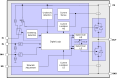
\includegraphics[width=0.5\linewidth]{Bilder/btn8982.pdf}
	\caption{Blockdiagramm der BTN8982 Halbbrücke \cite[S.4]{btn}}
	\label{fig:btn8982}
\end{figure}\noindent
Sie besteht aus einem \textit{p-channel highside MOSFET}, einem \textit{n-channel lowside MOSFET} und einem \textit{Driver IC}, die \textit{logic level inputs} unterstützt, wodurch der Anschluss an einen Microcontroller erleichtert wird. Die \textit{BTN8982} ist in einem Temperaturbereich von \SI{-40}{^\circ C} bis \SI{150}{^\circ C} einsetzbar und kann mit einer Versorgungsspannung von bis zu \SI{40}{V} betrieben werden, wobei diese im normalen Betrieb zwischen \SI{8}{V} bis \SI{18}{V} liegen sollte. Zusätzlich sind mehrere Schutzfunktionen integriert, beispielsweise ein Überstrom- und ein Übertemperaturschutz. Die \textit{BTN8982} besitzt acht Ausgänge, welche in \autoref{tab:Pinverteilung} aufgelistet und im Folgenden näher erläutert werden.

\begin{table}[H]
	\centering
		\captionabove{Pinverteilung Halbbrücken}
		\begin{tabular}{l p{2,5cm} p{8cm} p{3cm}}
			\textbf{Pin Nummer} & \textbf{Bezeichnung} & \textbf{Erläuterung} & \textbf{Anschluss an} \\ \hline
			1 & GND (Ground) & Erdung & Ground MCU \\
			2 & IN (Input) & definiert die Schalterstellung (1 = High Switch Mode; 0 = Low Switch Mode) & O-Pin MCU \\
			3 & INH (Inhibit) & 1: Betriebsmodus, 0: Schlafmodus & O-Pin MCU \\
			4, 8 & OUT (Output) & Ausgang der Brückenschaltung & Aktor \\
			5 & SR (Slew Rate) & Einstellen der Steigung der Spannungsantwort & Ground über Widerstand \\
			6 & IS (Status) & Strommessung \& Fehlererkennung & I-Pin MCU\\
			7 & VS (Supply) & Stromversorgung & Batterie\\
		\end{tabular}
	
	\label{tab:Pinverteilung}
\end{table}\noindent
Pin 1 ist der GND-Pin und bestimmt das Bezugsniveau der Versorgungsspannung, welche an Pin 7 angelegt wird. Ob Strom durch den highside MOSFET oder den lowside MOSFET fließt, wird durch Pin 2 (IN) bestimmt. Liegt eine 1 an fließt Strom durch den highside MOSFET, während bei einer 0 Strom durch letzteren fließt. Wird die Halbbrücke über ein PWM Signal geschaltet, geschieht dies über das Signal an diesem Pin. Der dritte Pin (INH) setzt die Halbbrücke in einen \textit{sleep-mode}, solange eine 0 anliegt. Somit kann die Halbbrücke nur genutzt werden, wenn eine 1 anliegt. Der \textit{sleep-mode} wird als Notaus verwendet, falls die Software einen kritischen Fehler detektiert (siehe \autoref{subsec:MOT}). Pin 4 und 8 (OUT) sind die Pins an die die Versorgungsspannung durchgeschaltet wird und stellen damit die direkte Schnittstelle mit dem Aktor da. Pin 5 (SR) bestimmt die Slew Rate des PWM Signals IN-Pin. Der sechste Pin (IS) ist für die Strommessung, sowie für die Meldung von Fehlern zuständig. Die Funktionsweise ist in \autoref{fig:IS_Pin} dargestellt.\\

\begin{figure} [H]
	\centering
	\includegraphics[width=0.7\linewidth]{Bilder/IS_Pin.pdf}
	\caption{Funktionsweise des IS \cite[S.18]{btn}}
	\label{fig:IS_Pin}
\end{figure}\noindent
Im normalen Operationsmodus (Current Sense Mode) liefert eine integrierte Stromquelle einen Strom $I_{is}$ der proportional zum durchgeschalteten Strom $I_{l}$ ist. Tritt ein Fehler auf wie zum Beispiel Übertemperatur oder Überstrom, schaltet die Halbbrücke in den Error Flag Mode. Hierbei wird die Stromquelle am IS-Pin gewechselt, welche einen konstanten Strom $I_{IS}$ liefert.  Dieser beträgt maximal \SI{6,5}{mA}. Der Proportionalitätsfaktor $k$ ist durch

\begin{equation}
k = \frac{I_{L1}-I_{L2}}{I_{IS}(I_{L2})-I_{IS}(I_{L1})}
\end{equation}\noindent
definiert und beträgt laut Datenblatt typischerweise 19.500. Messungen haben gezeigt, dass $k$ in der geschalteten H-Brücke unterhalb dieses Wertes liegt, sodass er als obere Abschätzung des geflossenen Stroms verwendet werden kann.
Die Spannungen an IN- und INH-Pins und somit auch die Funktionalität der H-Brücke wird durch einen hochgeschwindigkeits Leitungsverstärker/Puffer (\textit{CD74HCT125}) bereitgestellt. Leitungsverstärker sind elektronische Verstärkerschaltungen, die eingesetzt werden, um die Qualität elektrischer Signale zu verbessern \cite{Conrads2014}. Der schematischer Schaltplan des verwendeten Leitungsverstärkers und die zugehörige Logiktabelle in \autoref{fig:buffer} dargestellt. Der \textit{CD74HCT125} besitzt vier unabhängige Wege, die getrennt voneinander aktiviert werden können. Diese Aktivierung geschieht hierbei über ein \textit{Low Level} Spannungssignal am nOE-Pin. Low Level bedeutet, dass die Spannung maximal \SI{1,35}{V} betragen darf. Aufgrund des Platinendesigns \autoref{kap5} lässt sich dies recht problemlos bewerkstelligen, was neben der Hitzebeständigkeit und Schnelligkeit das Hauptargument für diesen Leitungsverstärker ist. Ist ein Weg aktiviert, sorgt ein \textit{High Level} Spannungssignal am Eingang (nA) dafür, dass die Versorgungspannung (VCC) an den jeweiligen Ausgang (nY) durchgeschaltet wird. In der ausgeführten Schaltung wird am VCC-Pin des \textit{CD74HCT125} eine Spannung von \SI{5}{V} angelegt. Die ersten drei Wege sind direkt mit GND verbunden, wodurch eine dauerhafte Aktivierung realisiert wird. Die ersten beide Wege sorgen für die Spannung an den IN-Pins der Halbbrücke, während der dritte Weg die INH-Pins versorgt. Die Eingänge sind dabei mit dem Microcontroller und die Ausgänge mit den Pins der Halbbrücke verbunden. Somit wird das PWM-Signal des Microcontrollers, welches eine maximale Spannung von \SI{3,3}{V} besitzt, auf ein PWM-Signal mit einer maximalen Spannung von \SI{5}{V} angehoben.

\begin{figure}[H]
	\begin{center}
		\noindent\begin{minipage}[h!]{0.45\textwidth} %Beginn der ersten Minipage
			\centering
			\includegraphics[height=0.85\textwidth]{Bilder/buffer.pdf}
		\end{minipage} %Ende der ersten Minipage
		\quad
		\begin{minipage}[h!]{0.45\textwidth} %Beginn der zweiten Minipage
			\centering
			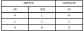
\includegraphics[height=0.3\textwidth]{Bilder/tabelle.pdf}
		\end{minipage} %Ende der zweiten Minipage
	\end{center}
	\caption{Schematischer Aufbau und Logiktabelle des CD74HCT125 Leitungsverstärkers \cite[S.2]{Buffer}}
	\label{fig:buffer}
\end{figure}\noindent
Die H-Brücke kann auch ohne einen Leitungsverstärker direkt mit dem Microcontroller verbunden werden, was zur Folge hätte, dass keine \SI{5}{V} sondern \SI{3,3}{V} Spannung an den Pins der H-Brücke anliegen. \autoref{fig:Strommessung} zeigt den geflossenen Strom durch den dabei angeschlossenen Aktor mit und ohne Leitungsverstärker bei variierenden PWM-Signalen. Es ist zu sehen, dass die Messung mit Geschalteten Leitungsverstärker deutlich symmetrischer sind, was auf eine bessere bidirektionale Schaltbarkeit schließen lässt. Außerdem sind die maximal durchgeschalteten Ströme größer. Dies lässt vermuten, dass die \SI{3,3}{V} nicht ausreichen um die Transistoren in den Halbbrücken vollständig schalten zu lassen. Dementsprechend wurde sich bei der endgültigen Schaltung für den Einsatz eines Leitungsverstärkers entschieden. 

\begin{figure} [H]
	\centering
	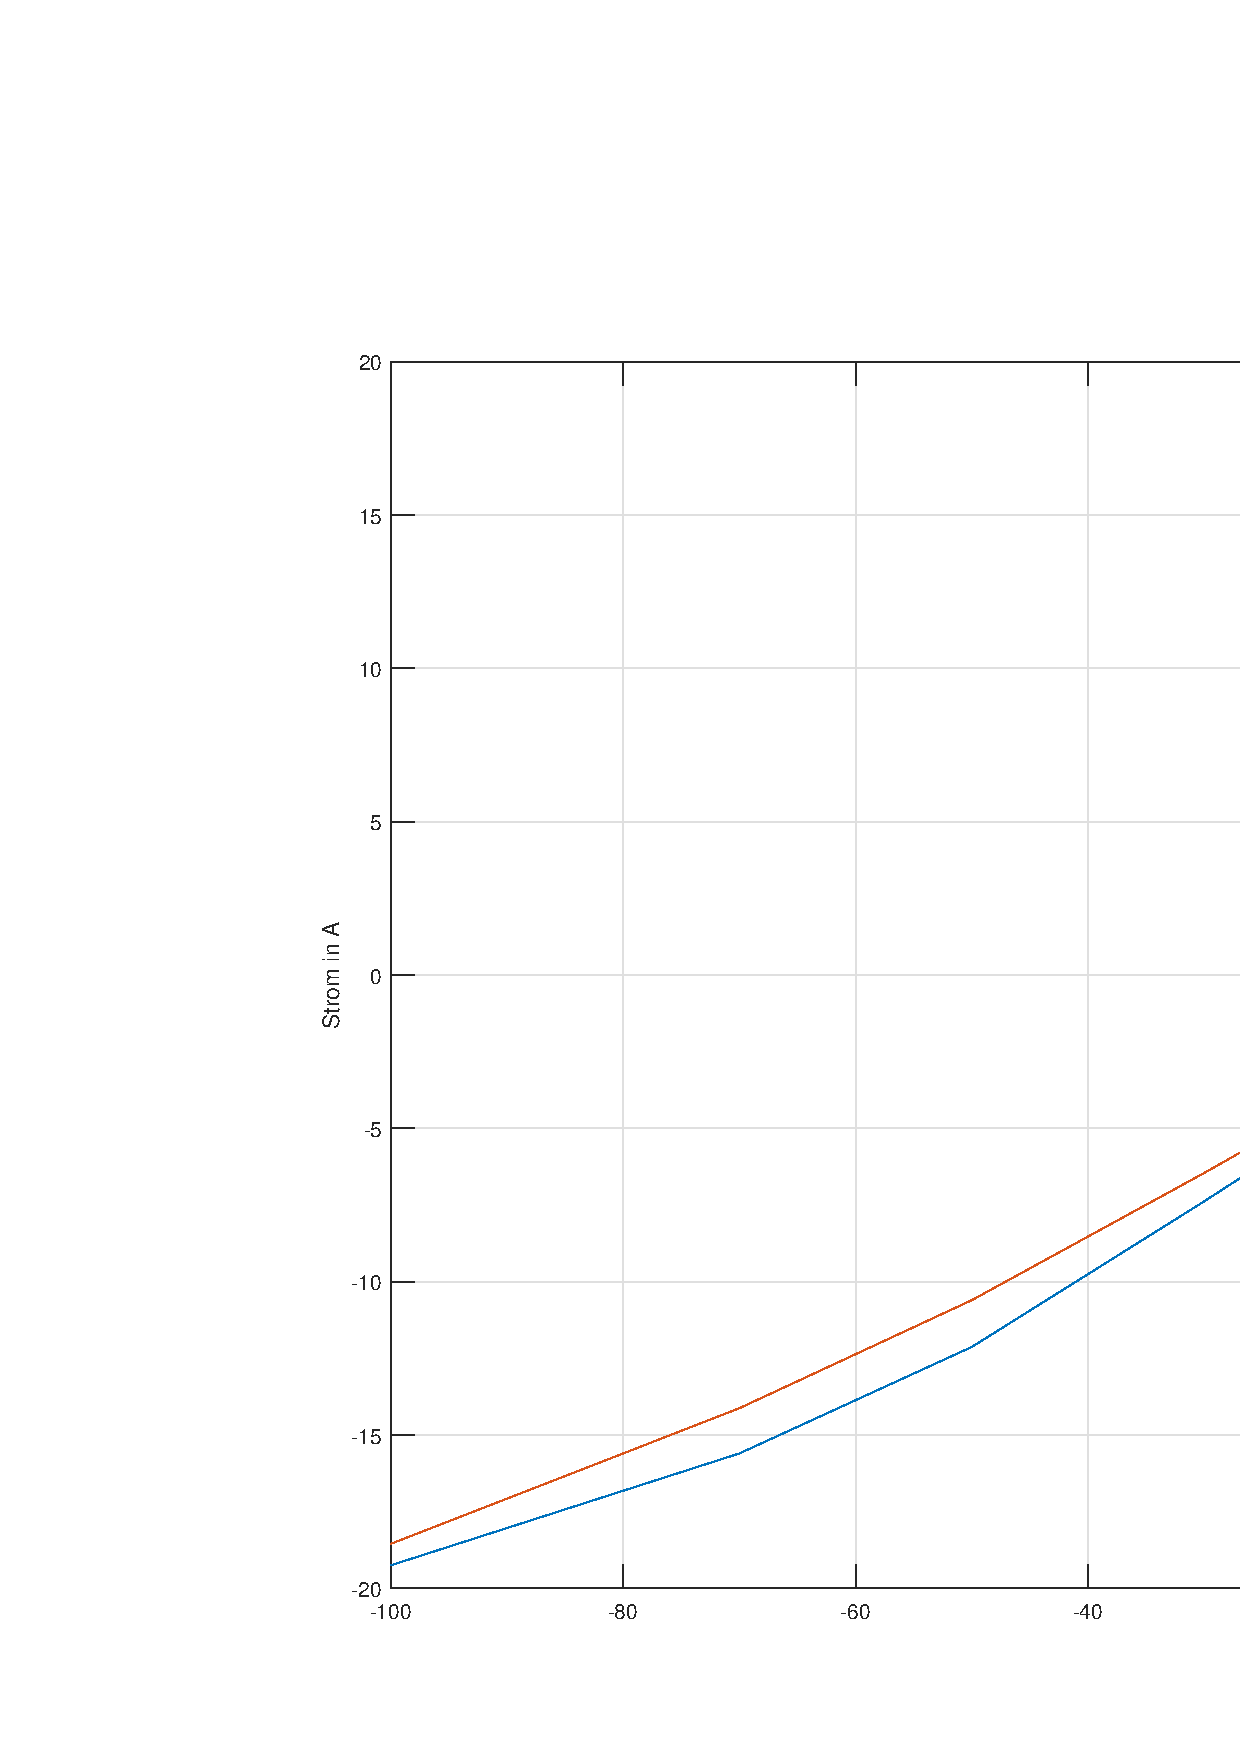
\includegraphics[width=0.8\linewidth]{Bilder/Strommessung.pdf}
	\caption{Strommessung mit und ohne Leitungsverstärker bei unterschiedlichen PWM-Signalen}
	\label{fig:Strommessung}
\end{figure}\noindent
Der schematische Aufbau der verwendeten H-Brücke ist in \autoref{fig:schematisch_hbruecke} zu sehen und wird im Folgenden genauer erläutert. Bei dem hier vorgestellten Aufbau wurde sich am Datenblatt der \textit{BTN8982}-Halbbrücken orientiert.

\begin{figure} [H]
	\centering
	\includegraphics[width=1\linewidth]{Bilder/schematisch_hbruecke.pdf}
	\caption{Schematischer Aufbau der H-Brücke}
	\label{fig:schematisch_hbruecke}
\end{figure}\noindent
An beiden Halbbrücken wird am VS-Pin die Versorgungsspannung angelegt. Nahe am jeweiligen VS-Pin ist ein \SI{100}{nF} Kondensator (CH1, CH3) gegen GND geschaltet, welcher die Schwankungen der Versorgungsspannung, z.B. verursacht durch andere Komponenten, glättet. Ob diese Spannung an die OUT-Pins durchgeschaltet wird, hängt von der Spannung an den IN- und INH-Pins ab. Die INH-Pins setzen die Halbbrücken in einen \textit{sleep-mode}, wenn an ihnen keine Spannung zwischen 3 und \SI{5,3}{V} angelegt ist. Sofern diese Spannung anliegt, sorgt der gleiche Spannungsbereich am IN-Pin dafür, dass die Versorgungsspannung an die OUT-Pins der Halbbrücke durchgeschaltet wird. Jede Halb-Brücke besitzt zwei solcher OUT-Ausgänge, wobei einer über einen Pin und der andere über eine große Fläche auf der Rückseite realisiert wird. Letzterer eignet sich besser zum Übertragen großer Ströme, weshalb dieser zur Aktoransteuerung verwendet wird.  Die IN- und INH-Pins werden über \SI{10}{k\Omega} Widerstände (R10, R11, R12, R13) mit den Ausgängen des Leitungsverstärkers verbunden. Diese Widerstände werden zum Schutz der digitalen Eingänge benötigt.
Die IS-Pins der Halbbrücke werden direkt mit dem Mikrocontroller verbunden. Parallel sind \SI{0,5}{k\Omega} (R9, R14), sowie ein  \SI{1}{nF} Glättungskondensator (C14, C15) gegen GND geschaltet. Diese Pins sind für die Sensorik der Halbbrücke verantwortlich. An ihnen ist eine Stromquelle angeschlossen, die einen zum durchgeschalteten Strom proportionalen Strom liefert. Abhänging von den gegen GND geschalteten Widerständen ergibt sich eine Spannung die vom Mikrocontroller gemessen und aus der der durchgeschaltete Strom berechnet werden kann. Da der Strom am IS-Pin maximal \SI{6,5}{mA} beträgt, resultiert durch einen \SI{0,5}{k\Omega} eine maximale Spannung von \SI{3,25}{V} am Mikrocontroller. Ein größerer Widerstand hätte eine größere Spannung zur Folge, wodurch eine Schädigung des Mikrocontrollers nicht mehr ausgeschlossen werden kann. 
Die Widerstände, die zwischen SR-Pins und GND geschaltet sind (R16, R17), bestimmen die Slewrate des durchgeschalteten Signals. Dieser darf laut Datenblatt zwischen \SI{0}{\Omega} und \SI{51}{k\Omega} liegen. Der Hersteller bietet zudem eine Simulation an, in der verschiedene Slew-Rate-Widerstände getestet werden können. Die Ergebnisse einer solchen Simulation mit den eingestellten Widerständen \SI{0}{\Omega}, \SI{10}{k\Omega} und \SI{51}{k\Omega} sind anhand des durchgeschalteten Stroms $I_{OUT}$ in \autoref{fig:Simulationsergebnisse} dargestellt. Es ist zu sehen, dass der durchgeschaltete Strom mit zunehmendem Widerstand abnimmt, die Welligkeit jedoch nahezu gleich bleibt. Allerdings gilt es zu beachten, dass die \textit{Electromagnetical Interference} (kurz: EMI) für kleinere Slew-Rate-Widerstände ansteigt. Ein Widerstand von \SI{10}{k\Omega} stellt dabei einen guten Kompromiss dar und liefert auch in realen Messungen sehr gute Ergebnisse.
\begin{figure} [H]
	\centering
	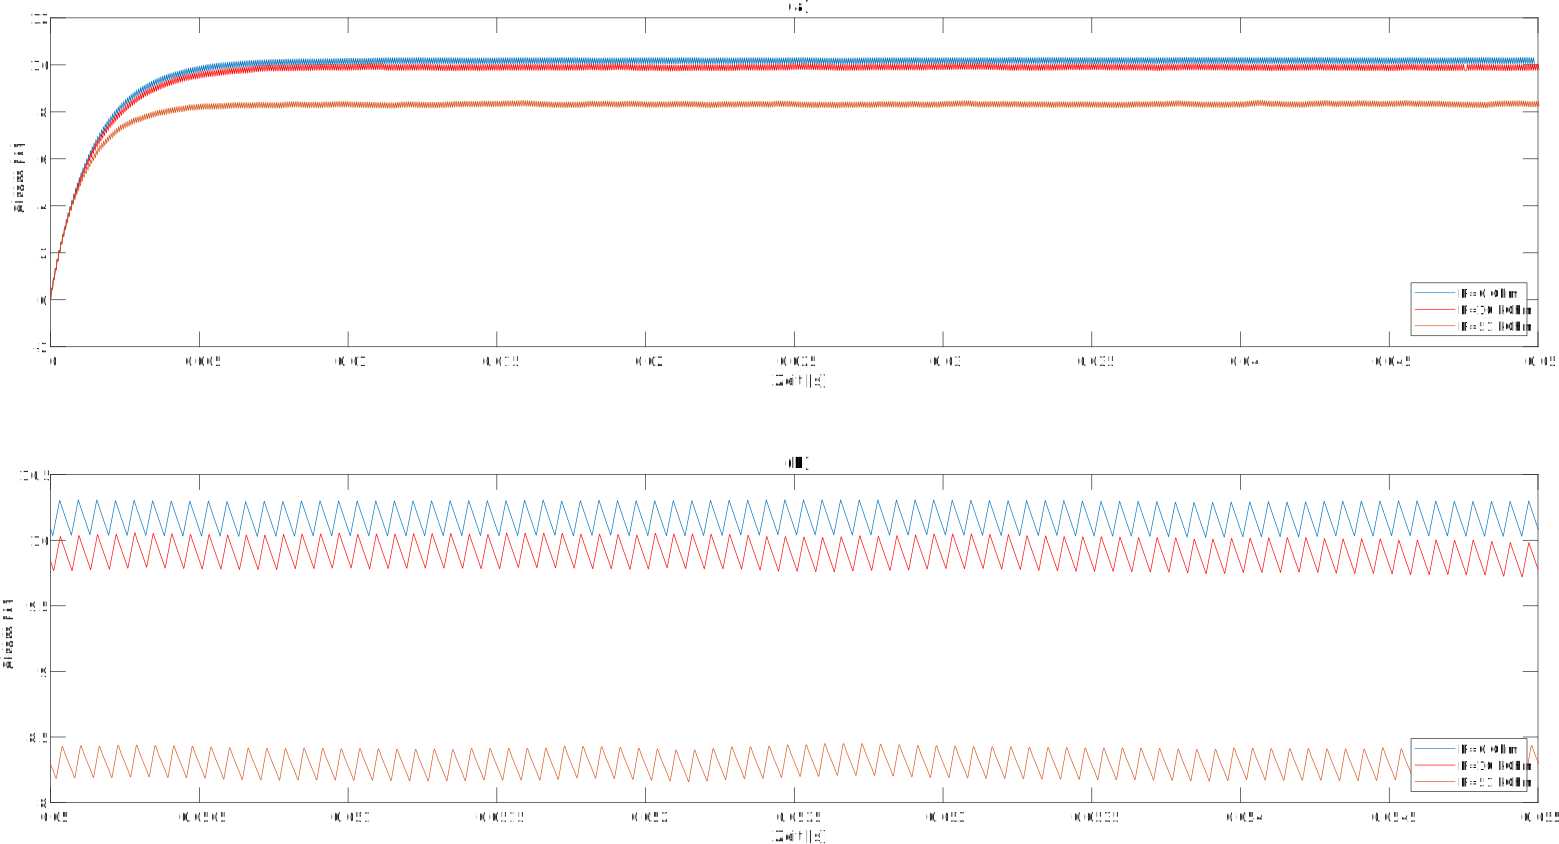
\includegraphics[width=1\linewidth]{Bilder/Simulationsergebnisse.pdf}
	\caption{(a):Simulationsergebnisse des durchgeschalteten Stroms über der Zeit aufgetragen; (b): Welligkeit des durchgeschalteten Stroms}
	\label{fig:Simulationsergebnisse}
\end{figure}\noindent
Bei der Simulation, sowie auch in der realen Anwendung, beträgt die Schaltfrequenz \SI{16}{kHz}. Dabei wurde sich an der vorangegangenen Arbeit orientiert, wobei auch höhere (\SI{20}{kHz}) und niedrige Frequenzen (\SI{10}{kHz}) getestet wurden. Höhere Schaltfrequenzen bieten prinzipiell den Vorteil, dass die Welligkeit des durchgeschalteten Stroms abnimmt. Allerdings steigt dabei auch die EMI. Der Unterschied der Welligkeit zwischen \SI{16}{kHz} und \SI{20}{kHz} ist jedoch vernachlässigbar klein, weshalb sich für die geringe EMI entschieden wurde. Im Gegensatz dazu ist bei \SI{10}{kHz} die Zunahme der Welligkeit deutlich zu beobachten.  

\section{Sensorik}
Die Sensorik des Gesamtsystems besteht aus einem Stromsensor, einem Temperatursensor und einem Lagesensor. Während die ersten beiden wichtige Kontroll- und Leistungsgrößen liefern, ist der Lagesensor essentiell für die Schaltvorgänge und damit die Funktionalität des Gesamtsystems. Der Stromsensor ist in den BTN8982 Halbbrücken integriert und ist bereits beschrieben. Die Funktionsweise und Verschaltung des Temperatur- und Lagesensors werden im folgenden erläutert. 

\subsection{Temperatursensor}\label{sub:temp}
Als Temperatursensor wird ein \textit{B57861S0103A039}-Thermistor verwendet. Dieser besteht aus einem Sensor und zwei \SI{350}{mm} langen Anschlusskabeln. Thermistoren sind elektrische Widerstände, deren Wert temperaturabhängig variiert. Dabei werden sie in die zwei Gruppen Heiß- und Kaltleiter aufgeteilt \cite{Stiny2015}. Da der \textit{B57861S0103A039}-Thermistor zur ersten Gruppe gehört, wird im folgenden ausschließlich auf diese eingegangen. Heißleiter besitzen einen negativen Temperaturkoeffizient (NTC), was bedeutet, dass ihr elektrische Widerstand sich mit steigender Temperatur reduziert. Dieser Zusammenhang ist allerdings hochgradig nichtlinear und kann durch 

\begin{equation} \label{eq:NTC}
R(T) = R_R \cdot e^{B\left(\frac{1}{T}-\frac{1}{T_R}\right)}  
\end{equation}
beschrieben werden mit der Referenztemperatur $T_R$, dem Widerstand $R_R$ bei der Referenztemperatur und dem Beta-Wert $B$. Als Referenztemperatur wird meistens \SI{25}{^\circ C} gewählt. Der Beta-Wert ist eine Materialkonstante, die üblicherweise zwischen \SI{1500}{K} und \SI{6000}{K} liegt \cite{Stiny2015}. Für den \textit{B57861S0103A039}-Thermistor beträgt der Widerstand $R_R$ \SI{10}{k\Omega} und der Beta-Wert $B$ \SI{3988}{K}. Der Betriebstemperatur liegt zwischen \SI{-55}{^\circ C} und \SI{155}{^\circ C}, was in den typischen Bereich für Heißleiter fällt \cite{Stiny2015}.\\
Eine mögliche Schaltung zur hochgenauen Temperaturmessung mittels Heißleitern ist die Wheatstonsche-Brückenschaltung (\autoref{fig:wheatstone}) bestehend aus drei ohmschen Widerständen und einem NTC-Thermistor \cite{Stiny2015}.

\begin{figure} [h]
	\centering
	
\includegraphics[width=0.4\linewidth]{Bilder/wheatstone.pdf}
	\caption{Wheatstone-Brückenschaltung nach \cite[S.12]{Weissgerber2018}}
	\label{fig:wheatstone}
\end{figure}\noindent
Solange die Brücke ausgeglichen ist, liegt keine Spannungsdifferenz zwischen $P_1$ und $P_4$ vor. Ändert sich der Widerstand des Thermistors, wird der ausgeglichene Zustand verlassen und es kommt zu einer Spannungsdifferenz, aus der der veränderte Widerstand des Thermistors bestimmt werden kann. Wird \autoref{eq:NTC} nach der Temperatur $T$ umgestellt, lässt sich daraus die aktuelle Temperatur berechnen. Aus Platzgründen auf der endgültigen Platine und da die hiermit erzielbare Genauigkeit nicht benötigt wird, ist stattdessen ein Spannungsteiler zum Einsatz gekommen. Dieser Spannungsteiler teilt den am Thermistor und an einem festen Widerstand abfallende Spannung und ist in \autoref{fig_ther_elek} dargestellt. Aus der Spannung, die am konstanten Widerstand $R_c$ abfällt, kann auf die Spannung geschlossen werden, die am Thermistor $R_t$ abfällt und somit auch auf dessen aktuellen Widerstand. Über \autoref{eq:NTC} ist dann ein direkter Zusammenhang zur gemessenen Temperatur gegeben.
Die Spannungsmessung findet im Mikrocontroller bzw. in dessen Analog-Digital-Convertern (ADC) statt. Dabei sind für eine möglichst exakte Messung mehrere Umstände zu beachten, die nun exemplarisch erörtert werden. Die Überlegungen gelten jedoch auch für die übrigen Spannungsteiler und ADCs. Im STM32F4 kommen \textit{successive approximation analog-to-digital converter} zum Einsatz, die eine Auflösung von bis zu \SI{12}{bit} liefern \cite{stmref}. Die Messdauer ist dabei konfigurierbar, entspricht jedoch mindestens für jedes Auflösungs-Bit und 3 zusätzliche Takte (12 + 3 Takte)\cite[S.397]{stmref}. Dieser Takt $f_{ADC}$ entspricht dabei nicht dem Kerntakt, sondern dem \textit{Advanced Peripheral Bus Clock} (APBC), der sich durch konfigurierbare Takt-Teiler vom Kerntakt unterscheidet. \\
Durch den Aufbau des ADC's bedingt, führen zu große Eingangswiderstände (bzw. Widerstandswerte im Spannungsteiler) zu großen Ungenauigkeiten. Dies ist umso kritischer je kürzer die Messdauer beträgt, da sich die interne Kapazität im ADC bei großen Eingangswiderständen nur langsam aufladen kann. Nach Ablauf der Abtastdauer sollte  jedoch die interne Kapazität auf die tatsächlichen Spannung am Eingangspin aufgeladen sein, sonst kommt es zu Abweichungen (siehe dazu auch \cite{ADC}, \cite{stm32}). ST stellt für den Mikrocontroller \autoref{eq:ADC} bereit, durch welche sich der maximale Eingangswiderstand 
\begin{equation} \label{eq:ADC}
R_{AIN} = \frac{(k-0,5)}{f_{ADC} C_{ADC} ln(2^{N+2})} - R_{ADC}
\end{equation}
abhängig der Messdauer berechnen lässt. Dabei entspricht $k$ den konfigurierten Messtakten pro Messung, $C_{ADC}$ der Kapazität des internen ADCs, $N$ der Auflösung und $R_{ADC}$ dem Schaltwiderstand des ADCs. Über $k$ und $f_{ADC}$ lässt sich dabei die Messdauer beeinflussen und somit die erlaubten Eingangswiderstände am Spannungsteiler beeinflussen. Für eine effektive Messdauer von \SI{2,7}{\mu s} muss der Eingangswiderstand unter \SI{31,355}{k\Omega} liegen, während bei einer Messdauer von nur \SI{1,5}{\mu s} nur Eingangswiderstände bis \SI{440,6}{\Omega} für hohe Genauigkeit zulässig sind. Der Nachteil niedrigere Widerstände im Spannungsteiler liegt jedoch in der Belastung des jeweiligen Sensorausgangs. Dort kann nur ein begrenzter Strom bereit gestellt werden. Daher bietet es sich an, eine Kapazität parallel zum Eingang des ADCs und somit zu $C_{ADC}$ zu schalten, die als Puffer für $C_{ADC}$ dient \cite{ADC}. Hier muss jedoch beachtet werden, dass eine weitere Kapazität zusätzlichen Bauraum, Kosten und Fehlerpotential zur Folge hat. Darüber hinaus werden schnelle Signaländerungen durch die RC-Zeitkonstante zum Auf-/Entladen des Kondensators ggf. herausgefiltert. Für den Thermistor werden keine kritischen Temperatursprünge erwartet, daher wird in diesem Fall eine zusätzliche Kapazität $C_c$ eingesetzt.\\
Auch durch einen Impedanzwandler, also eine Operationsverstärkerschaltung mit einer Spannungsverstärkung von $1$, lässt sich der Eingangswiderstand durch den Spannungsteiler kompensieren. Auch hier ergeben sich jedoch Nachteile durch benötigten Bauraum, anfallende Kosten, gesteigertes Fehlerpotential und zusätzliches Rauschen.\\
\begin{figure}[H]
	\centering
	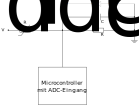
\includegraphics[width=0.5\linewidth]{./Bilder/fig_ther_elek}
	\caption{Schaltung zum Auslesen des Thermistors}
	\label{fig_ther_elek}
\end{figure}\noindent
Durch den Temperatursensor soll die Spulentemperatur im Tauchspulenaktor gemessen werden, da hier durch eine Überhitzung der Isolation Gefahrenpotential ausgeht. In der Umgebung der Spulen wird jedoch eine große Induktionswirkung erwartet, die die Genauigkeit der Spannungsmessung gefährden oder sogar ganz außerhalb des Messbereichs von \SI{0}{V} bis \SI{3,3}{V} liegen und somit die Funktionsfähigkeit des Mikrocontrollers gefährden \cite{stm32}. Eine Gegenmaßnahme stellt die Verseilung der Zuleiterkabel dar. Darüber hinaus kann durch die Schirmung der Kabel eine Schirmdämpfung erreicht werden, was die Induktionswirkung weiter reduziert \cite{Wolfsperger}. Falls trotzdem eine Spannung induziert wird, kann ein  Strom im mA-Bereich über interne Dioden im ADC abgeleitet werden \cite{stmref}. Um den Strom zu begrenzen, muss sich ein Widerstand zwischen induzierter Spannung und ADC-Eingang befinden. Eine weitere Methode den Pin vor einer Überspannung zu schützen, stellt eine Zener-Diode dar, die parallel zum Eingang des ADC's geschaltet wird (grau angedeutet). Hierbei ist jedoch darauf zu achten, dass auch im Normalbetrieb ein Kriechstrom durch die Diode fließt, der das Messergebnis verfälschen kann. \\
Um Probleme dieser Art zu umgehen, wurden auch alternative Sensorkonzepte in Betracht gezogen, die nicht über ein ADC ausgewertet werden. Diese haben sich jedoch als zu rechenaufwändig beim Auslesen erwiesen.

\subsection{Lagesensor}
Die Funktionsweise des PLCS-25M Sensors ist in \autoref{kap2} bereits erläutert worden. Der Sensor gibt demnach ein Spannungssignal aus, das nach \autoref{eq:Lage} in den Schaltgabelweg umgerechnet werden kann. Hierbei ist zu beachten, dass der Lagesensor mit \SI{5}{V} Gleichspannung betrieben wird und demnach der mögliche Ausgangsspannungsbereich zwischen \SI{0}{V} und \SI{5}{V} liegt, was außerhalb des gültigen Messbereichs der ADCs liegt. Über einen Spannungsteiler wird die Ausgangsspannung des Lagesensors demnach in den gültigen Messbereich übersetzt. Es gelten dabei bei der Auslegung des Spannungsteilers die gleichen Überlegungen wie in \autoref{sub:temp}. Um darüber hinaus eine Verbesserung der Positionsbestimmung zu erreichen, wird auch der komplementäre Ausgang des Lagesensors gemessen und entsprechend verrechnet. Der dadurch erreichte Genauigkeitsgewinn wird in \autoref{kap7} thematisiert.

\subsection{Sensorik Eingangsspannung}\label{eingangsspannung}
Um Fehlerzustände in der Spannungsversorgung feststellen zu können, ist ein einfacher Spannungsteiler zu entwerfen, anhand dessen die Eingangsspannung in einen für den ADC lesbaren Bereich gebracht wird. Es gelten die gleichen Überlegungen wie in \autoref{sub:temp}.


\chapter{Platinenentwurf}\label{kap5}
Im Folgenden wird die Gedankengänge und Einflüsse eingegangen, die zum endgültigen Platinendesign geführt haben, eingegangen. Dabei wird neben der reinen Platinenbetrachtung auch die Rahmenbedingungen erläutert.
\section{Elektronikgehäuse und Anforderungen an die Platinendimensionierung}
Die Platine wird in ein Gehäuse eingebettet, welches parallel zu und in Absprache mit dieser Arbeit entwickelt wurde. Die Anforderung, den Aktor durch die entwickelte Elektronik zu einem \textit{Smart Actuator} zu transformieren wird erfüllt, in
dem die Platine durch das Gehäuse am Aktorgehäuse verschraubt wird. \autoref{fig:gh1} zeigt schematisch die Lage der Platine (grün) im Gehäuse. In grau ist der Verbindungsstecker zu sehen, der abgedichtet im Gehäuse liegt. Anschließend wird ein Deckel montiert, wodurch die Elektronik von Schmutzpartikeln und anderen Umwelteinflüssen geschützt wird. Dieser ist aus Übersichtsgründen nicht abgebildet.

\begin{figure}[H]%
\centering
\includegraphics[width=300pt]{./Bilder/Elektronik_Gehauese_ver3}%
\caption{Derzeitiger Entwurf des Elektronikgehäuses}%
\label{fig:gh1}%
\end{figure}

Durch die Größe des Aktors ergeben sich Höchstmaße an das Platinengehäuse und die Platine selbst. Um ein Einbauen zu garantieren, dürfen die Außenmaße der Platine $\SI{88,8}{mm} \cdot \SI{50}{mm}$ nicht überschreiten. In diesem Fall war der Platz ausreichend, um alle nötigen Schaltungen und Funktionen auf der Platine zu verwirklichen. Als Ausweichlösung, falls die ebenen Maße nicht ausgereicht hätten war angedacht, die Elektronik auf zwei Platinen aufzuteilen (z.B. Logik- und Leistungsteil), und sie in zwei Ebenen parallel übereinander anzuordnen. Dies ist weiterhin denkbar, falls die Elektronik erweitert werden soll. Gelötete Teile auf der Platine, welche einen großen Bauraum nach oben benötigen sind vor allem der THT Kondensator mit \SI{1000}{\mu F} sowie die Wire-to-Board Reihenklemmen. Diese sind bereits auf der linken Seite (Steckerseite) der Platine angeordnet, sodass über der rechten Seite relativ unproblematisch eine zweite Platinenebene eingeführt werden könnte.
Da das Gehäuse aufgrund von kostengünstiger und einfacher Fertigung aus Kunststoff geplant und hergestellt wurde, muss eine Lösung gefunden werden um die Platine mit GND zu verbinden, zu kühlen und elektromagnetisch abzuschirmen. Es bietet sich an, eine Aluminiumplatte, die den Maßen der Platine entspricht, zwischen Platine und Gehäuse anzubringen. Dabei wird auf Aluminium zurückgegriffen, da es sich um ein kostengünstiges, leitfähiges Metall handelt, welches außerdem eine hohe Wärmeleitfähigkeit von \SI{204}{\frac{W}{mK}} besitzt \cite[S.4]{wuerth}. 
Durch das Loch in der Unterseite des Gehäuses, welches in \autoref{fig:gh2} zu erkennen ist, liegt die Aluminiumplatte, in dieser Darstellung grün eingefärbt, am Aktorgehäuse an. Das hat den Vorteil, dass die Platine Wärme an die Aluminiumplatte über Konduktion abgeben kann, welche wiederum ihre Wärme an das Aktorgehäuse aus Aluminium abgibt. Diese Wärmeübertragung soll durch Wärmeleitpaste beziehungsweise –kleber unterstützt werden. Diese Lösung erspart weitere externe Kühlkörper. Diese Methode hat die Einschränkung, dass nur die aluminiumfreie Seite der Platine bestückt werden darf, ansonsten müssen die betroffenen Bereiche in der Aluminiumplatte ausgespart werden. Da die Platine mit THT-Bauteilen teils auch auf der Unterseite verlötet werden musste, wurden die nötigen Aussparungen durch Bohrlöcher realisiert. 
\begin{figure}[H]%
\centering
\includegraphics[width=300pt]{./Bilder/Elektronik_Gehauese}%
\caption{Rückseite des Elektronikgehäuses zur Darstellung der Aktoranbindung}%
\label{fig:gh2}%
\end{figure}
Die vier Schrauben, mit denen Platine, Aluminiumplatte und Platinengehäuse am Aktorgehäuse verschraubt werden, sorgen zusätzlich für einen optimalen Wärmeübergang von Platine bis zum Aktor. Diese vier Schraubverbindungen plus zwei weitere Schraubverbindungen, welche Platine, Aluminiumplatte und Platinengehäuse verbinden, ermöglichen außerdem eine großflächige GND-Verbindung über die Aluminiumplatte. Die Auflageflächen der Schrauben sind jeweils auf GND-Potential gesetzt, sodass Schrauben und Platte auch dieses Potential annehmen.
Eine weiterer wichtiger Aspekt den es bei Platinengehäusen zu beachten gilt, ist die notwendige Abschirmung gegen Eintreten sowie Abstrahlung elektromagnetischer Strahlung. Das Kunststoffgehäuse ist dabei weniger geeignet als die Aluminiumplatte, die aufgrund der elektrischen Leitfähigkeit eine gute Basisschirmung besitzt \cite{bopla}. Für Kunststoffgehäuse wird im Allgemeinen eine Beschichtung aus Aluminium oder Kupfer empfohlen \cite{Gwinner2006}.

\section{Komponentenplatzierung auf der Platine}\label{sec:bau}
Beim Layout-Entwurf müssen mehrere Aspekte berücksichtigt werden: Die Platinenmaße und die Platzierung der GND-Schrauben müssen eingehalten werden und die Lokalität der Bauteile sollte gut durchdacht sein. Beispielsweise sollten die Halbbrücken nahe an der Spannungsversorgung platziert werden, um lange leistungsführende Leitungen zu verhindern. Weiterhin müssen die Leitungen der sensiblen Sensorik gegen elektromagnetische Rückwirkung geschützt werden. Beim engültigen Platinenentwurf, welcher in \autoref{fig:docu} zu sehen ist, ist die Lokalität der Leistungs-Bauteile, also der Halbbrücken mit den Bezeichnungen HB\_1 und HB\_2, deutlich von der Platzierung der Logikebene getrennt \cite[S.26]{emcdes}. Die Halbbrücken befinden sich auf der rechten Hälfte der Platine, nahe des Steckers, wodurch lange Leistungsleitungen vermieden werden können. Der Klemmblock (\textit{terminal block}) als Anschlussklemme für den Tauchspulenaktor ist ebenfalls nahe der Halbbrückenausgänge platziert, sodass auch die Ausgangsleitungen geringe Leitungslängen aufweisen. In \autoref{fig:docu} ist dieser Block mit der Bezeichnung TB\_1 gekennzeichnet. Der Kondensator zum Stabilisieren der Batteriespannung ist als C13 gekennzeichnet und ebenfalls nahe der Spannungsversorgung platziert. Aus Platzgründen mussten auch die Klemmblöcke für Temperatur- und externe Strommessung (J2 und J3) auf der rechten Platinenhälfte platziert werden. Da sich die leistungsführenden Leitungen jedoch auf die Mitte der Platine konzentrieren stellt dies kein Problem dar. In der linken Platinenhälfte befindet sich der Logikteil, welche den Mikrocontroller (\textit{STM32}), den CAN-Transciever (CAN\_T), den externen Taktgeber (QUARZ) und den Leitungsverstärker (\textit{CD74HCT}) umfasst. Neben diesen Bauteilen befindet sich ebenfalls die Spannungsregler für \SI{3,3}{V} und \SI{5}{V}, sodass bei der Spannungsversorgung für die ICs keine Probleme durch elektromagnetische Rückwirkungen auftreten und die Versorgungsleitungen zu den Bauteilen kurz gehalten werden kann. Bei der Platzierung der Bauteile spielt ebenfalls die Ausrichtung des Mikrocontrollers eine wichtige Rolle, sodass die benötigten Pins des Mikrocontrollers möglichst geringe Entfernungen zum jeweiligen Bauteil aufweisen. Dadurch kann ein Kreuzen der Signalleitungen vermieden und die Länge reduziert werden \cite[S.17]{emcdes}. So befinden sich beispielsweise die Ausgangspins CAN1\_RX und CAN1\_TX des Mikrocontrollers in \autoref{fig:docu} auf der oberen Seite des STM32 und die Leitungen zum CAN-Transciever (CAN\_T) können deshalb leicht verlegt werden. Die Leitungen für die H-Brücke sind auf der rechten Seite des Mikrocontrollers platziert, sodass sich diese leicht zum Leitungstreiber (CD74HCT) legen lassen. Die Pins für den externen Quarz befinden sich an der unteren Seite des STM32 und somit nahe des Schwingquarzes. Gerade bei diesem Bauteil ist die Entfernung zum Mikrocontroller möglichst gering zu halten und eventuelle Leitungskapazitäten zu verhindern \cite[S.31]{stmquarz}. Ebenfalls sollte der Taktgeber möglichst weit von den Halbbrücken entfernt platziert sein um Störungen durch Hochfrequenzsignalen vorzubeugen \cite[S.31]{stmquarz}.
Die Entkopplungskondensatoren der ICs sollten möglichst nahe an den Versorgungseingängen platziert werden, sodass beispielsweise die Entkopplungkondensatoren C10 und C11 nahe des VDD Pins des Mikrocontrollers (STM32) liegen \cite[S.17]{emcdes}.

\begin{figure}[H]%
\centering
\includegraphics[width=380pt]{./Bilder/docu}%
\caption{Platzierungsgrafik der Bauteile}%
\label{fig:docu}%
\end{figure}

\section{Dimensionierung der Leiterbahnen}
Um die Leiterbahnbreite für die Halbbrücken berechnen zu können, müssen die besonderen Gegebenheiten eines Schaltvorgangs beachtet werden. Es handelt sich um Kurzzeitbelastungen im zeitlichen Rahmen von maximal \SI{100}{ms} mit einer Stromstärke von maximal \SI{60}{A}. Aufgrund der Kurzzeitbelastung können die Leitungsquerschnitte deutlich geringer gewählt werden, als die Strombelastbarkeit nach der Norm IPC 2221 es für Leiterbahnen unter Dauerlast zulässt.\\
In einem stromdurchflossenen elektrischen Leiter entsteht Verlustleistung gemäß
\begin{align*}
P = I^{2}R
\end{align*}
da Energie aufgrund des Leitungswiderstandes 
\begin{align*}
R = \rho \frac{l}{A}(1+\alpha_{r}(T(t)-T_{r})
\end{align*}
dissipiert. Dieser Leitungswiderstand hängt sowohl von den materialabhängigen Konstanten $\rho$ (spezifischer Widerstand) und $\alpha_{r}$ (Temperaturkoeffizient zur Referenztemperatur $T_{r}$), als auch von der Leiterlänge $l$, dem Leiterquerschnitt $A$ und der Temperaturänderung $T(t)$ zur Referenztemperatur $T_{r}$ ab. Aufgrund der Erwärmung der Leiterbahn durch die Verlustleistung ist die Temperaturänderung zeitabhängig. Nach dem Stromwärmegesetz gilt für die Ableitung der Wärmeenergie nach der Zeit
\begin{align}
\label{eq:dif2}
\frac{\partial Q_{W}}{\partial t} = P = I^{2}\rho \frac{l}{A}(1+\alpha_{r}(T(t)-T_{r}).
\end{align}
Die Änderung der Wärmeenergie führt zu einer Änderung der Temperatur welche sich mittels Wärmekapazität $C$ beschreiben lässt
\begin{equation}
\label{eq:waermeaend}
 Q_{W} = (T(t)-T_{r})C_W,
\end{equation}
wobei sich die Wärmekapazität aus dem Produkt der materialabhängigen spezifischen Wärmekapazität $c$ und der Masse $m$ des Körpers zusammensetzt
\begin{equation}
C_W = c m.
\end{equation}
Daraus folgt für die zeitliche Ableitung von \autoref{eq:waermeaend} die Differentialgleichung
\begin{equation}
\label{eq:dif1}
\frac{\partial Q_W}{\partial t} = \frac{\partial ((T(t)-T_{r})C_W)}{\partial t} = \frac{\partial T(t)}{\partial t}C_W.
\end{equation}
Durch Einsetzen von \autoref{eq:dif2} in \autoref{eq:dif1} und der Notationsvereinfachung
\begin{align*}
\xi = I^2 \rho \frac{l}{A}(\alpha_r T_r-1)
\end{align*}
ergibt sich die Differentialgleichung erster Ordnung
\begin{equation}
\label{eq:dT}
T(t)I^2 \rho \frac{l}{A} \alpha_r-\frac{\partial T(t)}{\partial t}C = \xi .
\end{equation}
Die Differentialgleichung lässt sich mittels Exponentialansatz und der Anfangsbedingung $T(0) = T_r$ lösen, sodass sich eine Funktion der Temperatur in Abhängigkeit der Zeit ergibt
\begin{align*}
T(t) = \left(T_r-\frac{\xi}{I^2 \rho \frac{l}{A} \alpha_r}\right)e^{\frac{I^2\rho \frac{l}{A}\alpha_r}{C_W}t}+\frac{\xi}{I^2\rho \frac{l}{A}\alpha_r}
\end{align*}
woraus durch Einsetzen von $\xi$, $C_W$ und $m = \varrho l A$ folgt:
\begin{equation}
\label{eq:T}
T(t) = \left(T_r-\frac{\alpha_rT_r-1}{\alpha_r}\right)e^{\frac{I^2\rho\alpha_r}{A^2\varrho c}t}+\frac{\alpha_r T_r-1}{\alpha_r}
\end{equation}
Für den Anwendungsfall der Platinenauslegung wird jedoch der minimale Leiterquerschnitt bei maximal zulässiger Temperaturänderung benötigt, sodass die Gleichung umgestellt nach dem Leiterquerschnitt $A$
\begin{equation}
\label{eq:A}
A = I\sqrt{\frac{\rho\alpha_r t}{c\varrho \ln{\left(\frac{T(t)-\frac{\alpha_rT_r-1}{\alpha_r}}{T_r-\frac{\alpha_rT_r-1}{\alpha_r}}\right)}}}
\end{equation}
lautet. Mit \autoref{eq:A} lässt sich für eine bestimmte Belastungsdauer $t_i$ und der maximal zulässigen Endtemperatur der Platine $T(t_i)$ für einen beliebigen Stromfluss $I$ berechnen. Die Herleitung dieser Formel basiert auf der Annahme, dass die Leiterbahn keinen thermischen Austausch mit ihrer Umwelt erfährt und sich somit theoretisch ohne Begrenzung erhitzen kann. Nach dem Energieerhaltungssatz wird die Leiterbahn durch ihren Umgebungsraum und ihre Umgebungstemperatur begrenzt. Unter der Annahme, dass die Umgebungstemperatur durch Nutzung des Aktorgehäuses als Kühlkörper deutlich geringer ist als die maximal zulässige Leiterplattentemperatur ist die Leitungstemperaturabschätzung durch den Wärmeaustausch geringer als in \autoref{eq:T} berechnet. Der Leitungsquerschnitt nach \autoref{eq:A} ist somit überdimensioniert und kann gut als minimale Abschätzung genutzt werden.
\begin{figure}[h]%
\centering
\subfigure{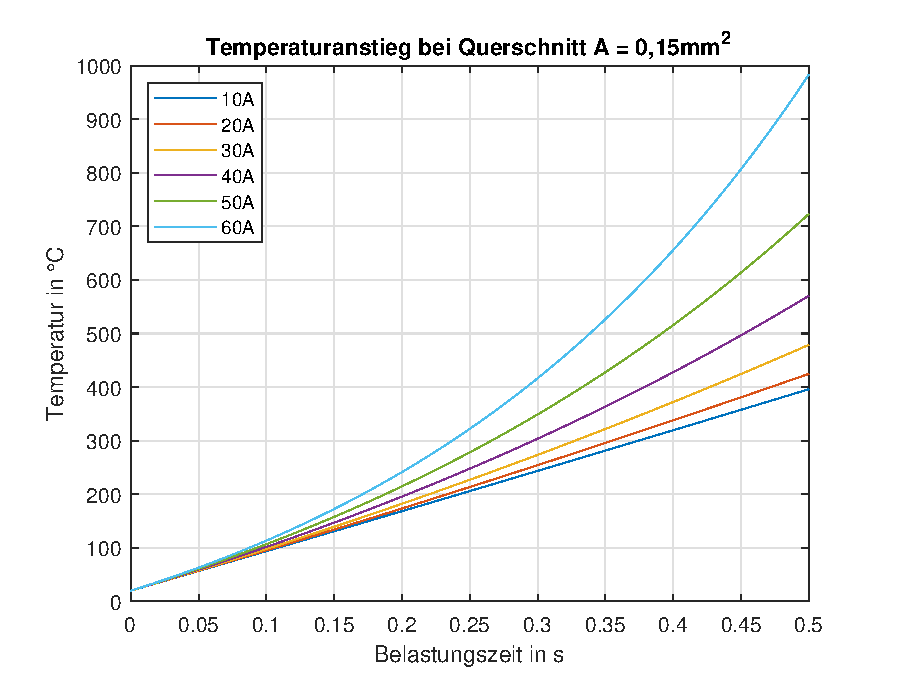
\includegraphics[width=247pt]{./Bilder/temp.eps}}
\subfigure{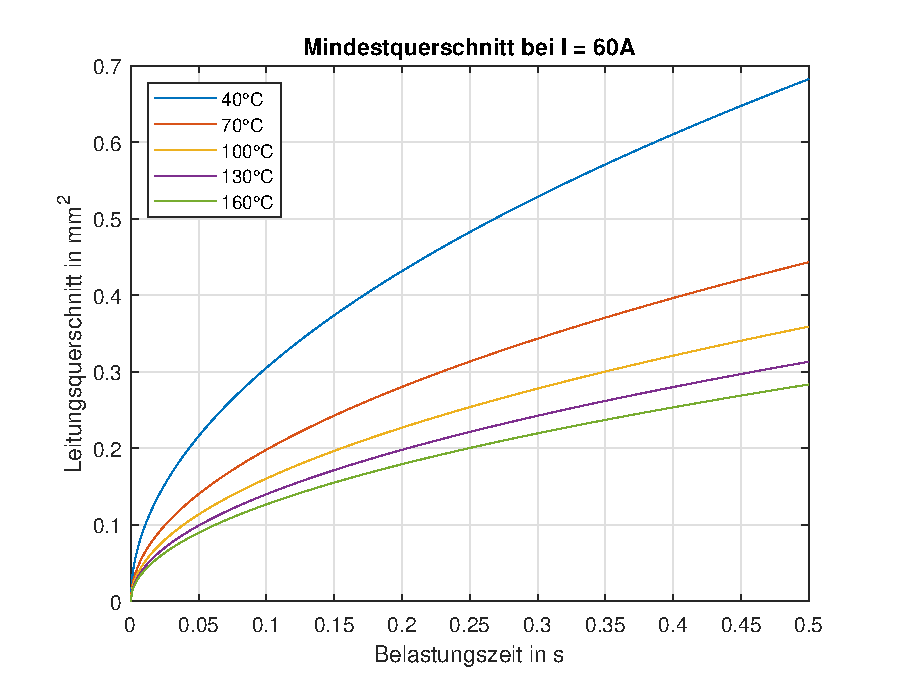
\includegraphics[width=247pt]{./Bilder/quer.eps}}
\caption{Dimensionierungsauswirkungen Temperatur und Leitungsquerschnitt}%
\label{fig:dimensionierung}%
\end{figure}\\
In \autoref{fig:dimensionierung} ist in der linken Abbildung der Temperaturanstieg über die Belastungsdauer bei verschiedenem Stromfluss und konstantem Querschnitt zu sehen. Es lässt sich erkennen, dass die Temperatur stärker über die Zeit ansteigt, je höher der Stromfluss über die Leiterbahn ist. Weiterhin ist der Steigungsverlauf exponentiell. In der rechten Abbildung ist der minimale Leitungsquerschnitt über die Belastungszeit bei konstantem Strom und verschiedenen zulässigen Maximaltemperaturen zu sehen. Der Verlauf des Leitungsquerschnittanstiegs ist logarithmisch und bei niedrigeren zulässigen Leitungsmaximaltemperaturen steigt der benötigte minimale Leitungsquerschnitt. 
\subsection{Anwendung auf realer Platine}
Die Kenndaten für die minimale Dimensionierung und die Kennwerte des Platinenmaterials sind in \autoref{tab:kennPl} beschrieben. Als Maximaltemperatur wurde dabei der Wert \SI{80}{^{\circ}C} gewählt. Der FR4-Kern der Platine ist nach Angaben des Herstellers für eine Temperatur bis zu \SI{135}{^\circ C} ausgelegt. Die lineare Temperaturabhängigkeit des Kupfers gilt annähernd im Bereich von -50...\SI{150}{^{\circ}C}\cite[S. 9]{Stiny2015}. Weiterhin ist die Anforderung an die Bauelemente, dass sie einen Temperaturbereich von mindestens -40...\SI{105}{^{\circ}C} abdecken. Um sich innerhalb dieser Bereiche zu bewegen und bei Temperaturausschlägen einen Sicherheitsfaktor zu berücksichtigen, sind die Leiterbahnen für die Maximaltemperatur von \SI{80}{^{\circ}C} auszulegen. Nach \autoref{tab:kennPl} ist für eine Kupferschichtdicke von \SI{70}{\mu m} eine Leiterbahnbreite von mindestens \SI{2,61}{mm} zu wählen. Beim Platinendesign ist diese aus Sicherheitsgründen zu \SI{3}{mm} gewählt, was einem maximalem Stromfluss von etwa \SI{69,1}{A} entspricht. Die Dimensionierung betrifft die Spannungsversorgungsleiterbahnen von der Batterie zu den Halbbrücken und die Leiterbahnen von den Halbbrücken zum Aktorklemmblock. Die restlichen Leiterbahnen auf der Platine sind für Dauerlast nach IPC 2221 auszulegen. Im Anhang findet sich ein Tabellenauszug nach IPC 2221 für die Strombelastbarkeit und eine Tabelle der Leistungsdaten der Platinenelemente, nach der die Leiterbahnen dimensioniert sind.
\begin{table}[H]%
\centering
\begin{tabular}{l l l l}
Kenngröße & Zeichen & Wert & Einheit\\ \hline
Temperaturkoeffizient Cu (20°C) & $\alpha_{20}$ & $3,93\cdot 10^{-3}$ &\SI{}{K^{-1}}\\
Spez. Widerstand Cu & $\rho$ & $1,721\cdot10^{-2}$ & \SI{}{\frac{\Omega\cdot mm^2}{m}}\\
Spez. Wärmekapazität Cu & c & 385 & \SI{}{\frac{J}{kg\cdot K}}\\
Dichte Cu & $\varrho$ & 8,92 & \SI{}{\frac{g}{cm^3}}\\
Referenztemperatur & $T_{20}$ & 20 &\SI{}{^\circ C}\\
Maximalstrom & $I_{max}$ & 60 & \SI{}{A}\\
Belastungsdauer & $t_i$ & 0,1 &\SI{}{s}\\
Maximaltemperatur & $T(t_i)$ & 80 & \SI{}{^\circ C}\\
Kupferschicht Dicke & d & $70\cdot 10^{-6}$ &\SI{}{m}\\
& & \\
resultierender Querschnitt & A & 0,1824 & \SI{}{mm^2}\\
resultierende Leiterbahnbreite & b & 2,6059 &\SI{}{mm}\\
\end{tabular}
\caption{Kenndaten Platine mit Kupferschicht}
\label{tab:kennPl}
\end{table}
\section{Routen der Platine}
Bei der letztendlichen Verlegung (\textit{routing}) der Leiterbahnen gibt es mehrere Aspekte zu beachten, die einerseits Einfluss auf die Elektromagnetische Verträglichkeit (\textit{EMV}), andererseits auch auf die Komplexität des Routingvorgangs haben.
\subsection{Design-Regeln und EMV}\label{sec:design}
Das Verlegen langer Leitungen sollte nach Möglichkeit vermieden werden um potentielle Störgrößen wie elektromagnetische Induktion und kapazitives Leitungsverhalten zu verringern \cite{haendschke}. Wie bereits in Abschnitt \autoref{sec:bau} erwähnt, sollten deshalb eine gewisse Lokalität der Bauteile eingehalten werden. Um die Leiterbahnen verlegen zu können sollten die Leiterplattenebenen (\textit{Layer}) abwechselnd verschiedene präferierte Verlegerichtungen aufweisen, sodass die Signale leicht an jeden Punkt der Platine verlegt werden können. In \autoref{fig:layer} ist schematisch der Aufbau einer zwei Layer Platine dargestellt. Im Falle einer gleichen Verlegerichtung kann es auftreten, dass sich die Signalleitungen auf keinem der vorhandenen Layer kreuzen können und somit unnötig lange Leitungen verlegt werden müssen \cite{haendschke}. Signale können zwischen den Platinen-Layern über Durchkontaktierungen (\textit{vias}) wechseln. Durchkontaktierungen sollten jedoch so selten wie möglich genutzt werden, da diese induktives Leitungsverhalten bewirken. In der Abbildung ist diese metallische Durchkontaktierung zwischen Layer 1 und Layer 2 exemplarisch dargestellt. Eine Signalleitung in Layer 1 kann, wenn sie mit der Metallfläche der Via verbunden ist, in Layer zwei weiter verlegt werden.
\begin{figure}[H]%
\centering
\includegraphics[width=300pt]{./Bilder/layer}%
\caption{Darstellung einer zwei Layer Platine inklusive Via}%
\label{fig:layer}%
\end{figure}
Prinzipiell können Platinen mit deutlich mehr Layer-Ebenen entworfen werden, zwei Layer Platinen werden jedoch bei industriellen Endprodukten aufgrund ihrer geringen Kosten präferiert \cite[S.13]{emcdes}. Im endgültigen Platinendesign wurde sich deshalb auch für eine zwei Layer Platine entschieden. Beim Verlegen der Leiterbahnen sollte weiterhin darauf geachtet werden, dass möglichst keine Winkel über \SI{45}{Grad} auftreten, da diese unerwünschte Reflektionen hervorrufen können \cite[S.17]{emcdes}. Bei wichtigen Signalleitungen sollte darauf geachtet werden, dass der Abstand zu anderen Leitungen größtmöglich ist, um eine Rückwirkung der Leiter aufeinander zu minimieren. Zur Verbesserung der Schirmung der Signalleitungen gegeneinander wird häufig eine GND-Leitung zwischen den Signalleitungen verlegt, welche die Rückwirkung verringert \cite[S.45]{Franz2012}.
Wenn diese Grundregeln der Leiterbahnplanung bekannt sind, gibt es nach \cite[S.12]{emcdes} drei Schritte, die zu einer fertigen Platine führen:
\begin{itemize}
	\item Komponentenauswahl und Platzierung (siehe \autoref{ch:komp} und \autoref{sec:bau})
	\item Entwurf des Versorgung- und Entkopplungskonzepts
	\item Verlegen der Signalleitungen
\end{itemize}
Nachdem in \autoref{sec:bau} die Bauteilplatzierung erläutert wurde, ist in \autoref{fig:logb} der erste Entwurf der Logikebene der Platine mit Versorgungskonzept und verschalteten Abblockkondensatoren zu sehen. Die Versorgungsleitungen werden dabei vor den Signalleitungen verlegt, da diese je nach Leistungsführung in ihrer Breite angepasst werden müssen. Die Logikebene beschränkt sich in dem Entwurf auf den STM32 und einen CAN-Transciever mit Pin-Ausgängen zur Ansteuerung der H-Brücke. Im dritten Schritt werden dann die Signalleitungen verlegt. Die Abbildung ist nur exemplarisch erstellt und wurde nie in Auftrag gegeben. Sie soll lediglich eine Nachvollziehbarkeit der Herangehensweise bewirken.
\begin{figure}[H]%
\centering
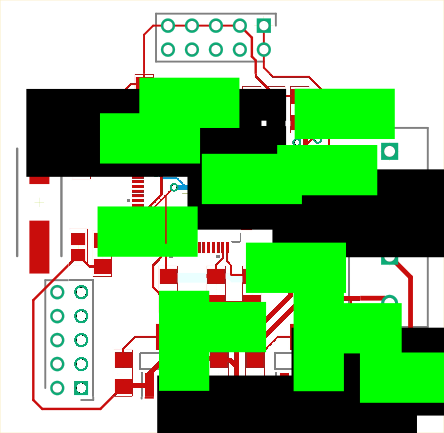
\includegraphics[width=250pt]{./Bilder/logb}%
\caption{Logikboard zur Endplatine inklusive Versorgungsleitungen}%
\label{fig:logb}%
\end{figure}
Üblicherweise werden zur Verbesserung der EMV nach dem Verlegen der Leiterbahnen die freien Platinenflächen zur Abschirmung auf GND Niveau gesetzt, welche als Teilmassenflächen bezeichnet werden. In der einschlägigen Literatur wird darauf hingewiesen, dass diese mit Vorsicht behandelt werden müssen, da Resonanz- und Antenneneffekte auftreten können. Um diesen Effekten vorzubeugen müssen die Masseflächen so gut wie möglich miteinander verbunden werden, sodass diese bei richtigem Anschluss die Schirmungsfunktion übernehmen \cite[S.166]{Franz2012}. Bei einem Layout mit 4 oder mehr Layern wird empfohlen vollständige GND-Layer und Versorgungslayer einzuführen, sodass eine optimale Abschirmung erfolgen kann \cite[S.172]{Franz2012}. Ein weiterer Effekt der im Bezug auf GND-Flächen betrachtet werden sollte ist das so genannte GND-Bouncing. Dieser Effekt tritt auf, wenn man keine gute Verbindung zwischen den GND-Flächen hat und somit unterschiedliche GND-Potentiale entstehen. Verstärkt wird dieser Effekt von Switching-ICs, also aktiven Bauteilen mit Schaltcharakteristiken, welche teilweise beim gleichzeitigen Umschalten von 1 nach 0 einen Zeitpunkt aufweisen, zu dem VCC und GND kurzgeschlossen sind und sich somit das GND Potential kurz anhebt \cite[S.1]{gndbnc}. Aufgrund dieses Effektes sollte die GND-Fläche so gut wie möglich verbunden sein um das GND Potential gleichmäßig zu halten. Problematisch ist dabei auch nicht zwingend wenn es kein geschlossenes GND-Layer gibt, solange die GND-Verbindungen der Ebenen sich außreichend überlappen und über Durchkontaktierungen gut verbunden sind \cite[S.172]{Franz2012}. Zur Abschirmung der aktiven Bauelemente gegen Welligkeiten der Spannungsversorgung werden wie in \autoref{ch:komp} erwähnt Abblockkondensatoren verwendet. Dabei sollten möglichst SMD Bauteile genutzt werden um entstehende parasitäre Induktivitäten zu verringern \cite[S.34]{emcdes}. Als Abschirmung gegen von außen autretende elektromagnetische Felder sei die Schirmwirkung von Kühlkörpern oder Gehäuseteilen aus Metall hervorgehoben \cite[S.22]{Franz2012}.

\subsection{Leiterbahnverlegung des Entwicklungsboards}
Die Verlegung der Leiterbahnen auf dem endgültigen Entwicklungsboard geschieht nach den zuvor definierten Designregeln, wobei aufgrund des geringen Platzes häufig Kompromisse eingegangen werden müssen. Das Entwicklungsboard weist 2 Layer auf, welche der Anordnung aus \autoref{fig:layer} entsprechen und im Folgenden über die Bezeichnung Top-Layer (obere Leiterebene) und Bottom-Layer (untere Leiterebene) gekennzeichnet werden. Grundanforderungen an die Platine ist die Positionierung der GND-Löcher, durch welche die Platine mittels Schrauben über das Aktorgehäuse mit GND verbunden ist. In \autoref{fig:top} und \autoref{fig:bot} ist das fertige Top-und Bottom-Layer der Platine zu sehen. Problematisch für das Einhalten der Designregeln ist hauptsächlich die Platzierung der Halbbrücken und der mittleren Schraubenlöcher, welche den Platz für die Signalleitungen von dem Mikrocontroller in Richtung Platinenstecker stark begrenzen. Die präferierte Verlegerichtung auf dem Top-Layer ist vertikal gewählt um die jeweiligen ICs über kurze Wege ohne große Leitungsverluste erreichen zu können. Dabei liegen CAN-Transciever und Leitungsverstärker oberhalb und der externe Schwingquarz unterhalb des Mikrocontrollers, was optimal für die präferierte Leitungsrichtung ist. Problematisch ist die Leitungsverlegung in Richtung der Halbbrücken und des Steckers, da der Spalt zwischen Schraubloch und Halbbrücke in der oberen Platinenhälfte durch die Versorgungsspannung belegt ist. 
\begin{figure}[H]%
\centering
\includegraphics[width=400pt]{./Bilder/top2}%
\caption{Darstellung des Top-Layers}%
\label{fig:top}%
\end{figure}
Die präferierte Verlegerichtung des Bottom-Layers ist horizontal ausgerichtet, sodass diese Leiterebene hauptsächlich zum Erreichen der Halbbrücken und des Steckers genutzt wird. Bei Betrachtung von \autoref{fig:bot} fällt jedoch auf, dass der Platz für die Leitungen sehr begrenzt ist und somit ein Teil der horizontalen Leiterbahnen auf das Top-Layer verlegt werden musste. Eine weitere wichtige Aufgabe beim Verlegen der Leiterbahnen ist die Reduktion elektromagnetischer Rückwirkung, wobei sich an die Methoden aus \autoref{sec:design} gehalten wird. Potentielle Gefahrenquelle der Rückstrahlung sind die Halbbrücken, da diese beim Schalten mit PWM-Signal Stromimpulse in hohen Frequenzen durchschalten können. Wichtige Signalleitungen wie die der Sensorik sind also möglichst weit von den Flächen mit der Bezeichnung V\_MOT\_PL und V\_MOT\_MIN (Halbbrücken Ausgänge) zu verlegen. Aufgrund des Platzmangels lassen sich die Signalleitungen der Sensorik nicht vollständig aus dem Einflussgebiet der Halbbrücken entfernen, sind jedoch von diesen so weit wie möglich entfernt verlegt. Bei genauerer Betrachtung der Layer fällt auf, dass jedoch trotzdem Signalleitungen nahe des Einflussgebietes der Halbbrücken verlaufen. Diese Leiterbahnen sind hauptsächlich die Leiterbahnen der SWD-Verbindung, also der Programmierschnittstelle der Platine. Daher stellt dies kein Problem dar, da die Platine nicht im laufenden Aktorbetrieb programmiert wird und somit die Lokalität im Einflussgebiet der Halbbrücken kein Hindernis darstellt. Die Leitungen zur Ansteuerung der Halbbrücken HB1\_IN und HB2\_IN sollten ebenfalls nicht im direkten Einflussgebiet liegen, damit die Halbbrücken vom Mikrocontroller noch problemlos angesteuert werden können. Als Konzept zur Abschirmung elektromagnetischer Rückwirkung wurde bereits der Einsatz von Abblockkondensatoren erwähnt, der eine wesentliche Rolle spielt. Neben diesen sind die freien Boardflächen auf beiden Layern auf GND-Potential gesetzt um damit ebenfalls Schirmungseffekte erzielen zu können. Diese sind zwar auf beiden Layern nicht optimal zusammenhängend, es wurde aber darauf geachtet über Durchkontaktierungen eine stabile gemeinsame GND-Fläche zu erhalten, welche gegen GND-Bouncing geschützt ist. Die GND-Flächen werden ebenfalls über die Aluminiumplatte und den Aktor auf ein gleichmäßiges Potential gezogen. Neben den EMV-Maßnahmen sollte auch die Wärmeentwicklung der Bauteile berücksichtigt werden. Aufgrund des hohen Stromflusses stellen die Halbbrücken besondere Anforderungen an die Kühlung. Insbesondere in Transistorschaltvorgängen innerhalb der Halbbrücke während denen ein Teil der Versorgungsspannung an den Transistoren abfällt und somit nach $P = U\cdot I$ erhöhte Wärmeenergie entsteht. Um die Halbbrücken unter ihrer kritischen Temperatur halten zu können, muss die entstehende Wärme abgeführt werden. Dies kann beispielsweise durch Durchkontaktierungen (\textit{Thermische Vias}) unter den kritischen Bauteilen erreicht werden. Über die Thermischen Vias vergrößert sich die zusammenhängende Metallfläche auf der sich die Wäre ausbreiten kann in das Bottom-Layer, und kann somit gut über den anliegenden Aluminium-Körper abgeführt werden.
\begin{figure}[H]%
\centering
\includegraphics[width=400pt]{./Bilder/bottom2}%
\caption{Darstellung des Bottom-Layers}%
\label{fig:bot}%
\end{figure}

\newpage
\section{Fertigung}
In \autoref{fig:platop} und \autoref{fig:plabot} ist die Platine nach dem Fertigungsprozess zu sehen. Als Kenndaten für die Fertigung wurde eine Leiterbahndicke von \SI{70}{\mu m} festgelegt. Als Kern wird ein FR4 Verbundwerkstoff mit einer Dicke von \SI{1,5}{mm} verwendet. Gut zu sehen sind auf den fertigen Leiterplatten auch die thermischen Vias, welche in das Lötpad von HB\_1 und HB\_2 eingelassen sind.
\begin{figure}[H]%
\centering
\includegraphics[width=400pt]{./Bilder/pla_top2}%
\caption{Top-Layer nach dem Fertigungsprozess}%
\label{fig:platop}%
\end{figure}
\begin{figure}[H]%
\centering
\includegraphics[width=400pt]{./Bilder/pla_bot2}%
\caption{Bottom-Layer nach dem Fertigungsprozess}%
\label{fig:plabot}%
\end{figure}
\chapter{Software}\label{kap6}
\chapter{Analyse und Performance}\label{kap7}
\section{Produktvergleich mit Anforderungsliste}\label{vergleich}
Um das Endresultat im Kontext der zuvor definierten Anforderungen analysieren zu können, wird sich auf die Anforderungsliste aus \autoref{kap1} berufen, welche aus Übersichtsgründen in \autoref{tab:Anforderungsliste2} noch einmal abgebildet ist.\\ 
Im Rahmen der Arbeit wurde eine zuvor eingerichtete \textbf{CAN-Schnittstelle} zum Senden von CAN-Nachrichten genutzt. Dazu werden die Signale in die nach \autoref{CANNachrichten} definierten Befehle unterschieden, sodass sich eine sinnvolle und benutzerfreundliche Menge an übermittelbaren Nachrichten ergibt. Es ist sowohl möglich die benötigten Schaltbefehle zu übermitteln, als auch Statusmeldungen über Übertemperatur, Überspannung etc. zu empfangen. Damit ist die Festforderung erfüllt.\\
Um eine \textbf{nichtflüchtige Kalibrierung} zu realisieren, werden die Daten der durchgeführten Kalibrierung in den Flash-Speicher abgelegt. Aufgrund der Speichertechnologie ist dieser nichtflüchtig, womit die Kalibrierungsdaten auch bei Unterbrechung der Versorgungsspannung des Mikrocontrollers erhalten bleiben. Bei erneuter Kalibrierung werden die alten Kalibrierungsdaten überschrieben.\\
In \autoref{kap7} sind die Plots zu der Regelung des Tauchspulenaktors zu finden, anhand derer eine Abschätzung der \textbf{Schaltzeiten} gewonnen werden kann. In den Plots ist zu sehen, dass zwischen Empfangen des Schaltbefehls und Einlegen des Ganges weniger als \SI{55}{ms} vergehen. Damit ist die Bereichsforderung von Schaltzeiten \SI{<100}{ms} erfüllt.\\
Bei der \textbf{selbstständigen Fehlererkennung} wurden im Zusammenspiel zwischen \autoref{ch:komp} und \autoref{kap6} Erkennungsstrategien für Überstrom, Temperaturüberschreitung und Fehler in der Eingangsspannung implementiert. Überstrom lässt sich über die IS-Pins der H-Brücken detektieren, dessen Funktion in \autoref{sec:hbridge} genauer erklärt wird. Zur Überprüfung einer Temperaturüberschreitung wird ein Temperatursensor im Aktorgehäuse verbaut, der in \autoref{sub:temp} beschrieben ist. Die Überprüfung der Eingangsspannung erfolgt nach \autoref{eingangsspannung}. Die Aufgabe der Dekalibrierungserkennung ließ sich im Rahmen des jetzigen Versuchsstandes nicht realisieren, könnte aber nach einer Erweiterung des Prüfstandes möglich sein. Im Falle eines betriebenen Motors ließe sich detektieren, ob dieser im Leerlauf betrieben wird, was der Getriebestellung im Neutralgang entspricht. Wird ein Lastmoment detektiert, was sich von dem Referenzlastmoment unterscheidet, ließe sich ein Kalibrierungsfehler erkennen, da in diesem Fall ein Gang eingelegt ist. Das Referenzlastmoment entspricht dem Leerlaufmoment. Diese Überlegung zur Detektion eines Kalibrierungsfehlers ist zu prüfen, womit diese Festforderung nur in Teilen erfüllt wurde.\\
Als Anforderungen an die \textbf{Schnittstellen} sind CAN-Kommunikation, Versorgungsspannungen von \SI{8-16}{VDC} und der Aufbau einer Programmierschnittstelle genannt. Diese Schnittstellen sind alle erfolgreich implementiert worden, was in \autoref{ch:komp} beschrieben ist. Als Programmierschnittstelle wurde sich für eine SWD-Verbindung via ST-Link/V2 entschieden, sodass Updates und Bugfixes problemlos über den Stecker möglich sind. Zusätzlich wurde die Möglichkeit einer UART Kommunikation offen gehalten, sodass diese ebenfalls für Debugging benutzt werden kann. Diese Festforderung ist in allen Punkten erfüllt.\\
Der Wunsch über \textbf{Wartbarkeit} wurde erfüllt. Die Sicherungen laufen über einen externen Sicherungsblock, welcher im späteren Einsatz im Fahrzeug dessen Sicherungsblock entsprechen soll. Die Platine ist bei derzeitigem Elektronikgehäusestand entnehmbar und somit austauschbar. Bei Softwareproblemen muss dies jedoch nicht erledigt werden, da die Programmierschnittstelle über den Stecker nach außen geführt wird. \\
Mit einer Baugröße von 88,8x\SI{50}{mm} weist die Platine eine kompakte Baugröße auf und ist somit für den Einbau in einem Smart Actuator geeignet. Im Vergleich mit dem zuvor verwendeten Motortreiber Arduino IBT2 Motortreiber, welcher eine Platinenfläche von 50x\SI{50}{mm} besitzt, weist die Platine weniger als die doppelte Fläche auf, obwohl Logik, CAN-Kommunikation, Spannungsregler, Sensorik und EMV-Maßnahmen ebenfalls darauf platziert sind. Damit ist diese Bereichsforderung erfüllt. \\
Die \textbf{Temperaturbeständigkeit} wird in \autoref{ch:komp} behandelt und die Auswahl der Bauteile nach diesem Kriterium berücksichtigt. Um dieser Anforderung gerecht zu werden, ist die Mehrheit der Bauelemente nach dem AEC-Q Standard ausgewählt worden. Alle verwendeten aktiven und passiven Bauteile entsprechen so den Forderungen an einen Betriebstemperaturbereich von -40...\SI{105}{^\circ C}.\\
In der Regelung des Tauchspulenaktors tritt \textbf{Überschwingen} auf, was in \autoref{reglerergebnisse} dokumentiert ist. Als maximal zulässiger Wert der Überschwingung wird \SI{1}{mm} festgesetzt. Ab einem Überschwingen von \SI{2}{mm} aus dem Neutralgang heraus, ist von einem unabsichtlichen Gangwechseln auszugehen. Somit entspricht diese Forderung einer Sicherheit von zwei. Die Messergebnisse weisen Überschwingweiten von \SI{0,4}{mm} auf, daher ist ein unbeabsichtigter Gangwechsel ausgeschlossen. Die Bereichsforderung ist damit erfüllt.\\
Die \textbf{Standby-Leistungsaufnahme} beträgt in etwa \SI{1,38}{W}, da zur Versorgung des Mikrocontrollers und der restlichen Bauteile ein Standby-Strom von etwa 100mA fließt.\\
Nach \autoref{schaltgabelkraft} ist zu erkennen, dass über Gegenbestromung der Spule eine Gegenkraft zur Massenträgheit (Lorentzkraft) aufgebaut wird. Darüber wird die \textbf{Schaltgabelkraft} am Anschlag minimiert.\\
Die Forderung nach \textbf{Effizienz} konnte nicht zuverlässig überprüft werden, wobei nach \autoref{sec:analyse_stellsignal} davon ausgegangen werden kann, dass sie erfüllt ist.
\begin{table}[h]
	\centering
	\captionabove{Anforderungsliste}
		\begin{tabular}{l|p{5cm}|p{7cm}|c}
			\textbf{Relevanz} & \textbf{Anforderung} & \textbf{Erläuterung} & Erfüllt?\\ \hline
			& &\\
			FF & Benutzerfreundliche Kommunikation durch CAN Schnittstelle & Empfang von Befehlen, Senden von Statusmeldungen & \checkmark\\ \hline
			FF & Nichtflüchtige Kalibrierung & Eine Kalibrierung ist nur einmalig und zur Rekalibrierung notwendig& \checkmark\\ \hline
			BF & Schaltzeit & < \SI{100}{ms} (Latenz zwischen Senden des Befehls und vollständig ausgeführtem Gangwechsel)& \checkmark\\ \hline
			FF & Selbstständige Fehlererkennung & Überstrom, Temperatur, Eingangsspannungsbereich, Dekalibrierung& (\checkmark) \\ \hline
			FF & Schnittstellen & CAN, \SI{8-16}{VDC} Versorgung, Programmierschnittstelle (für Updates \& Bugfixes)& \checkmark \\ \hline
			W & Wartbarkeit & Sicherung wechseln im eingebauten Zustand& \checkmark\\ \hline
			BF & kompakte Baugröße & 88,8x\SI{50}{mm}&\checkmark \\ \hline
			BF & Effizienz (gemittelt über einen Schaltvorgang) & elektrischer Wirkungsgrad > \SI{90}{\%} & ?\\ \hline
			FF & Temperaturbeständigkeit & bis \SI{105}{^\circ C}& \checkmark \\ \hline
			BF & Aktorüberschwingen & Toleriert, solange kein unbeabsichtigter Gangwechsel $\rightarrow$ \SI{<1}{mm}& \checkmark
			\\ \hline
			W & Schaltgabelkraft am Anschlag & möglichst gering& \checkmark \\ \hline
			FF & Standby & Standbyleistungsaufnahme < \SI{2}{W}& \checkmark \\ \hline
		\end{tabular}
	\label{tab:Anforderungsliste2}
\end{table}
\section{Kostenaufstellung}
Die Materialkosten für die fertige Platine inklusive aller Bauteile belaufen sich bei einer einzigen Platine auf \SI{80,26}{\euro}. Bei einer Stückzahl von 100 kann der Preis bereits auf \SI{33,51}{\euro} gesenkt werden, während die Bauteilkosten bei einer Fertigung von 1000 Platinen nochmal auf \SI{24,68}{\euro} sinken. Diesen großen Preisunterschied verursacht vor allem die unbestückte Platine selbst, die bei Bestellung von einer einzigen \SI{38,5}{\euro} kostet und bei einer Bestellung von 1000 Stück nur noch \SI{0,82}{\euro}. \autoref{tab:Preisliste} zeigt die verwendeten Bauteile und deren Anzahl sowie den kumulierte Preis pro Bauteilart (Anzahl des Bauteils multipliziert mit dem Einzelpreis) für jeweils eine Fertigung von einer Platine, von 100 Platinen und von 1000 Platinen. Die Nettopreise stammen dabei von den Anbietern, bei denen die Komponenten jeweils eingekauft wurden.
\begin{table}[h]
	\centering
	\captionabove{Preisliste}
\begin{tabular}{ l   l   c   c   c }
	Anzahl & Bauteil & Bauteilpreis & Bauteilpreis 100+ & Bauteilpreis 1000+\\ \hline
	1 & Platine & \SI{38,5}{\euro} & \SI{2,39}{\euro} & \SI{0,82}{\euro}\\
	\  & \  & \  & \  & \  \\
	1 & Mikrocontroller & \SI{10,66}{\euro} & \SI{7,79}{\euro} & \SI{6,58}{\euro} \\
	2 & Halbbrücken & \SI{6,56}{\euro} & \SI{5,96}{\euro} & \SI{5,04}{\euro}\\
	1 & Leitungstreiber & \SI{0,62}{\euro} & \SI{0,35}{\euro} & \SI{0,25}{\euro} \\
	1 & CAN Transceiver & \SI{2,82}{\euro} & \SI{2,28}{\euro} & \SI{1,51}{\euro} \\
	1 & Voltage Regulator \SI{3,3}{V} & \SI{0,34}{\euro} & \SI{0,16}{\euro} & \SI{0,10}{\euro} \\
	1 & Voltage Regulator \SI{5}{V}& \SI{0,34}{\euro} & \SI{0,16}{\euro} & \SI{0,10}{\euro} \\
	\  & \  & \  & \  & \  \\
	1 & Klemmblock & \SI{1,16}{\euro} & \SI{1,07}{\euro} & \SI{0,91}{\euro} \\
	2 & Klemmblock & \SI{0,74}{\euro} & \SI{0,62}{\euro} & \SI{0,53}{\euro} \\
	1 & Steckverbinder & \SI{0,04}{\euro} & \SI{0,04}{\euro} & \SI{0,04}{\euro} \\
	1 & AMPSEAL Automotive Steckverbinder & \SI{7,09}{\euro} & \SI{6,22}{\euro} & \SI{5,23}{\euro}\\
	\  & \  & \  & \  & \  \\
	1 & Quarz & \SI{0,61}{\euro} & \SI{0,36}{\euro} & \SI{0,38}{\euro} \\
	21 & Widerstände & \SI{4,88}{\euro} & \SI{3,05}{\euro} & \SI{1,68}{\euro}\\
	21 & Kondensatoren & \SI{5,91}{\euro} & \SI{3,06}{\euro} & \SI{1,50}{\euro}\\
	\  & \  & \  & \  & \  \\
	\  & \textbf{Gesamtpreis} & \textbf{\SI{80,26}{\euro}}  & \textbf{\SI{33,51}{\euro}}  & \textbf{\SI{24,68}{\euro}}  \\
\end{tabular}
	\label{tab:Preisliste}
\end{table}\noindent
Die gesamte Preisauflistung für die Stückzahlen 1, 100 und 1000 inklusive der einzelnen Widerstände und Kondensatoren, sowie die Händlerlinks zu allen Bauteilen befindet sich im Anhang.
In nachfolgenden Abbildungen wird die Verteilung der Kosten auf die verschiedenen Bauteilgruppen dargestellt. Die Bauteile wurden unterteilt in die Platine, die passiven Bauteile (Kondensatoren, Widerstände und Schwingquarz), die ICs (Mikrocontroller, Spannungsregler, CAN Transceiver, Leitungstreiber, Halbbrücken) sowie die Stecker, die die Schnittstellen nach außen darstellen. 

\begin{figure}[H]
\begin{minipage}[h]{0.5\textwidth}
\includegraphics[width=\textwidth]{./Bilder/Platinenkosten.pdf}
\end{minipage}
\begin{minipage}[h]{0.5\textwidth}
\includegraphics[width=\textwidth]{./Bilder/Platinenkosten-tausend.pdf}
\end{minipage}
\caption{Aufteilung der Kosten für die Stückzahlen 1 (links) und 1000 (rechts)}
	\label{fig:LDO}
\end{figure}\noindent
Es ist zu erkennen, dass die Platine bei geringen Stückzahlen ungefähr die Hälfte der Kosten ausmacht, während sie bei hohen Stückzahlen fast gar nicht mehr ins Gewicht fällt. Bei hohen Stückzahlen sind der größte Kostenfaktor die ICs. 
Ein Preisvergleich mit direkter Konkurrenz fällt schwer, da es wenig äquivalente Produkte auf dem Markt gibt, jedoch können die beiden vorherig am Prüfstand verwendeten Motortreiber zum Vergleich gezogen werden, die nur einen Teil der Platinenfunktionen abdecken. Der Kaufpreis des Motorcontrollers MDC1460 des Herstellers RoboteQ liegt bei ca. \SI{260}{\euro} (bei über vierfachem Bauraum), der Kaufpreis des Arduino IBT\_2 Motortreibers liegt bei circa \SI{15}{\euro}. Zu bemerken ist, dass sich die Kosten der Platine auch mit einem mit einzurechnenden Gewinnaufschlag innerhalb des Preisrahmens der beiden Motortreiber bewegt, obwohl sie deutlich mehr Funktionen aufweist.

\section{Platinendesign-Analyse}\label{sec:platan}
Die Platine erfüllt für den derzeitigen Aktor die Aufgaben Positionsregelung bei Schaltvorgängen, Überwachung der Umgebung (Temperatur, Eingangsspannung, Ausgangsstrom) und die Kommunikation mittels CAN-Nachrichten. Bisher sind keine Probleme mit EMV aufgetreten, sodass die Sensorik auch bei Ansteuerung der Halbbrücken funktioniert und die CAN-Kommunikation erhalten bleibt. Die Anforderung an eine kompakte Baugröße wird mit 88,8x\SI{50}{mm} erfüllt. Eine einfache Handhabung in der Peripherie wird über den Anschlussstecker erreicht. Im Falle von Softwareupdates lässt sich der Betriebstecker leicht entfernen und die Updates über den Programmierstecker flashen, was in \autoref{sec:stecker} genauer behandelt wird. Sollten im Betrieb nach Einführen des neuen Aktors trotz der Schirmungsmaßnahmen Probleme mit EMV auftreten, so wird empfohlen das Platinendesign wie in \autoref{app:4layer} auf ein 4-Layer Design zu erweitern, um wie in \autoref{kap5} beschrieben, zusätzliche GND-Planes einfügen zu können. Weiterhin bleiben die LDOs der \SI{3,3}{V} und \SI{5}{V} Schiene zu beobachten, da diese beim Anschluss der Autobatterie relativ viel Wärme abgeben müssen um auf die jeweiligen Spannungsebenen zu regeln. Derzeit sind keine Probleme damit aufgetreten jedoch kann das Verhalten im Dauerbetrieb noch nicht vollständig abgeschätzt werden. Falls keine Probleme auftreten wird empfohlen diese auch bei Einführung eines 4-Layer Designs beizubehalten, da die LDOs konstante Spannungen ohne switching Charakteristiken liefern. Bei Problemen könnte ein Buck-Spannungsregler statt des \SI{5}{V} LDOs eingeführt werden, welcher von Batteriespannung auf die \SI{5}{V} regelt. Für die \SI{3}{V} könnte weiterhin ein LDO verwendet werden, welcher als VCC die \SI{5}{V} des Buck-Spannungsreglers nutzt. Damit wäre die Stabilität der \SI{3}{V} Versorgung für die ADC-Genauigkeit gesichert und das Problem entstehender Wärmeverluste reduziert. Allerdings könnte in dieser Verschaltung die Genauigkeit des Lagesensors nicht auf dem aktuellen Niveau garantiert werden, da dieser an die \SI{5}{V} angeschlossen ist und der Buck-Spannungsregler weniger konstante Spannungen ausgibt als ein LDO. 

\section{Regelergebnisse} \label{reglerergebnisse}
In \autoref{fig:shift_gear2} und \autoref{fig:shift_toneutral} sind die exemplarisch gemessenen Positionsverläufe, Regelabweichungen und Stellgrößen für das Schalten von Gang 2 zu Neutral und umgekehrt aufgetragen. Das Schalten von und nach Gang 1 wird nicht betrachtet, da der verbaute Synchronring die Regelung bei einer Drehzahl $n=0$ zu stark behindert.\\
Die Messungen wurden 20 mal durchgeführt, sodass eine Reproduzierbarkeit der Ergebnisse sichergestellt werden konnte. In den Abbildungen ist jeweils zum Zeitpunkt $t=0$ ein Sollwertsprung zu sehen. Die Sollwerte sind mit roten Linien gekennzeichnet und betragen für den zweiten Gang \SI{10}{mm} und Neutral \SI{0}{mm}. Für beide wurde ein Toleranzband festgelegt, dass \SI{10}{\%} der Sprunghöhe zwischen den Gängen entspricht. Der verwendete PID-Regler mit Störgrößenkompensation wurde in \autoref{regler} beschrieben.

\subsection{Schalten in Gang 2}

Für das Schalten in Gang 2 ist in \autoref{fig:shift_gear2} ein Überschwingen von \SI{380}{\mu m} zu beobachten. Dies kann allerdings auf die lose Befestigung des Lagesensors im Prüfstand zurückgeführt werden. Der Schaltvorgang bringt den ganzen Prüfstand kurzzeitig zum Schwingen, sodass der Lagesensor eine zusätzliche relative Bewegung zur Läuferstange erfährt. Die Sollposition wird erstmals nach \SI{42}{ms} erreicht und verlässt das Toleranzband nach einer Dauer von \SI{54}{ms} nicht mehr. In dem Verlauf der Stellgröße zeigt sich, dass für den Schaltvorgang das maximale PWM-Signal bei \SI{63}{\%} liegt und somit ein großer Anteil der möglichen Stromdurchschaltung gar nicht ausgenutzt wird. Die Stellgröße bleibt nahezu konstant, bis ca. \SI{2}{mm} vor dem Erreichen der Sollposition. Anschließend fällt sie kurzzeitig ins Negative, bevor sie bei \SI{0}{\%} einpendelt.  

\subsection{Schalten in Neutral}
Bei diesem Schaltvorgang zeigt \autoref{fig:shift_toneutral} ein erstes Überschwingen von \SI{288}{\mu m} über den Sollwert. Auch dieses Überschwingen kann durch die Bewegung des Sensors erklärt werden. Die Sollwertvorgabe wird nach \SI{42}{ms} zum ersten Mal erreicht und dessen Toleranzband wird nach \SI{50}{ms} nicht mehr verlassen. Die Stellgröße springt zu Beginn des Schaltvorgangs auf ein PWM-Signal von \SI{-72}{\%}, was anschließend betragsmäßig bis zu einer Regelabweichung von \SI{1,4}{mm} auf einen Wert von \SI{-28}{\%} abnimmt. An dieser Stelle springt das PWM-Signal in den niedrigen positiven Bereich, bevor es bei \SI{0}{\%} einpendelt.

\subsection{Diskussion der Regelergebnisse}\label{diskreg}
Die beiden Schaltvorgänge erreichen ihren Sollwert und die zugehörige stationäre Genauigkeit in unter \SI{50}{ms}, was die Anforderungen von einer Schaltzeit \SI{\leq100}{ms} klar erfüllt. Für die stationäre Genauigkeit ist die korrekte Positionierung des Lagesensors von entscheidender Bedeutung. Diese Postion bleibt allerdings nicht über alle Schaltvorgänge gleich, aufgrund der losen Halterung und den Erschütterungen des Prüfstands. Abhilfe könnte hier eine besserer Fixierung schaffen, wodurch die Regelergebnisse weiter verbessert werden könnten. Aber auch unter Annahme, dass die Überschwingungen nicht auf den Lagesensor zurückzuführen sind, stellen sie aufgrund ihrer geringen Größe (\SI{\leq400}{\mu m}) kein Problem dar. Erst ab einem Überschwingen von \SI{\geq1}{mm} wäre in der Neutralstellung die Gefahr des unabsichtlichen Schaltens in einen anderen Gang gegeben.\\
In den Verläufen der Stellgrößen ist zu erkennen, dass der Aktor ab ca. \SI{1-2}{mm} nicht mehr beschleunigt, sondern leicht abgebremst wird.\\
Mit der erreichten stationären Genauigkeit sind die Bedingungen für eine erfolgreiche Implementierung eines Haltereglers erfüllt. Dabei wird der Positionsregler durch einen anderen Regler abgelöst, sobald die Position das Toleranzband für eine bestimme Zeit nicht mehr verlässt. Die Aufgabe des neuen Reglers besteht dann lediglich darin die Postion zu halten, bis ein neuer Schaltbefehl erfolgt. Hauptproblem für diesen Regler ist der Haftgleiteffekt, welcher auf der Tatsache beruht, dass der Haftreibungskoeffizient größer als der Gleitreibungskoeffizient ist \cite{Bowden2001}. 

\begin{figure} [H]
	\centering
	\includegraphics[width=1\columnwidth]{Bilder/shift_gear2_test.pdf}
	\caption{Position, Regelabweichung und Stellgröße für das Schalten in Gang 2}
	\label{fig:shift_gear2}
\end{figure}

\begin{figure} [H]
	\centering
	\includegraphics[width=1\linewidth]{Bilder/shift_toneutral.pdf}
	\caption{Position, Regelabweichung und Stellgröße für das Schalten in Neutral}
	\label{fig:shift_toneutral}
\end{figure}

\subsection{Schaltgabelkraft am Anschlag}\label{schaltgabelkraft}
In \autoref{fig:aktor_anschlag} ist ein Schaltvorgang von Neutral in Gang 2 und die zugehörige Strommessung des Aktors aufgetragen. Zu sehen ist, dass beim Erreichen der Sollgröße zum Zeitpunkt $t$ = \SI{0,1316}{s} nur etwa \SI{0,1}{A} im Aktor fließt. Das bedeutet, dass die Lorentzkraft der Spule auf den Läufer gemäß \autoref{eq:lorentz} keine nennenswerte Kraft auf den Aktor ausübt. Somit wirkt auf den Läufer zu diesem Zeitpunkt fast ausschließlich die Kraft aufgrund seiner Massenträgheit. Nach dem Übertreten des Läufers der Sollposition reagiert die Regelung durch Gegenbestromung, sodass die Massenträgheit durch die Lorentzkraft gebremst wird und der Läufer in Richtung Sollposition gebracht wird. Die Anschlagskraft wird somit minimiert.

\begin{figure} [H]
	\centering
	\includegraphics[width=1\linewidth]{Bilder/aktor_anschlag2.pdf}
	\caption{Strommessung im Schaltvorgang von Neutral in Gang 2}
	\label{fig:aktor_anschlag}
\end{figure}

\section{Analyse des Stellsignals}\label{sec:analyse_stellsignal}
In \autoref{fig:spannungsverlaeufe} sind die Spannungsabfälle an den Aktorklemmen bei verschiedenen PWM-Signalen dargestellt. Zusätzlich ist der jeweils zugehörige Spannungsverlauf der Versorgungsspannung der Platine aufgetragen. Zu sehen ist, dass die Spannung der Batterie immer sinkt, sobald die H-Brücken die Spannung an den Aktor durchschaltet und anschließend wieder steigt. Diese Schwankung ist für größer werdende PWM-Signale aufgrund des steigenden Stroms ausgeprägter. Neben den zu beobachtbaren Schwankungen, fällt auch das Gesamtniveau der Batteriespannung für steigende PWM-Signale. Bei einem PWM-Signal von \SI{30}{\%} beträgt die Versorgungsspannung noch ca. \SI{13}{V} im durchgeschalteten Zustand, während sie bei \SI{70}{\%} nur noch \SI{10,5}{V} beträgt. Die Spannung am Aktor und die anliegende Batteriespannung weisen in allen drei Fällen im durchgeschalteten Zustand lediglich eine geringe Differenz auf, woraus gefolgert werden kann, dass in diesem Zustand die H-Brücke einen minimalen Widerstand bzw. einen sehr hohen Wirkungsgrad aufweist. Werden die gemessenen Spannungsverläufe über eine Periode (\SI{62,5}{\mu s}) integriert und anschließend mit dem nach \autoref{fig:Strommessung} nahezu konstant geflossenen Strom multipliziert, ergibt sich die dem Aktor zugeführte Leistung. Für $\text{PWM}=\SI{30}{\%}$ beträgt diese \SI{25,86}{W}, für $\text{PWM}=\SI{50}{\%}$ \SI{64,32}{W} und für $\text{PWM}=\SI{70}{\%}$ \SI{104,96}{W}. Dies entspricht lediglich einer Annäherung, da die minimale Stromwelligkeit aus \autoref{fig:Simulationsergebnisse} vernachlässigt wird und der Strom als konstant angenommen wird.
Auch die \textit{slew rate} lässt sich durch den Spannungsverlauf des Aktors ermitteln. Diese bestimmt sich aus dem Quotient des Spannungsdifferenz und der dafür benötigten Zeit. In allen drei Fällen resultiert eine \textit{slew rate} von ca. \SI{5}{V/\mu s}. Das ermittelte Verhalten entspricht den Erwartungen.


\begin{figure} [h]
	\centering
	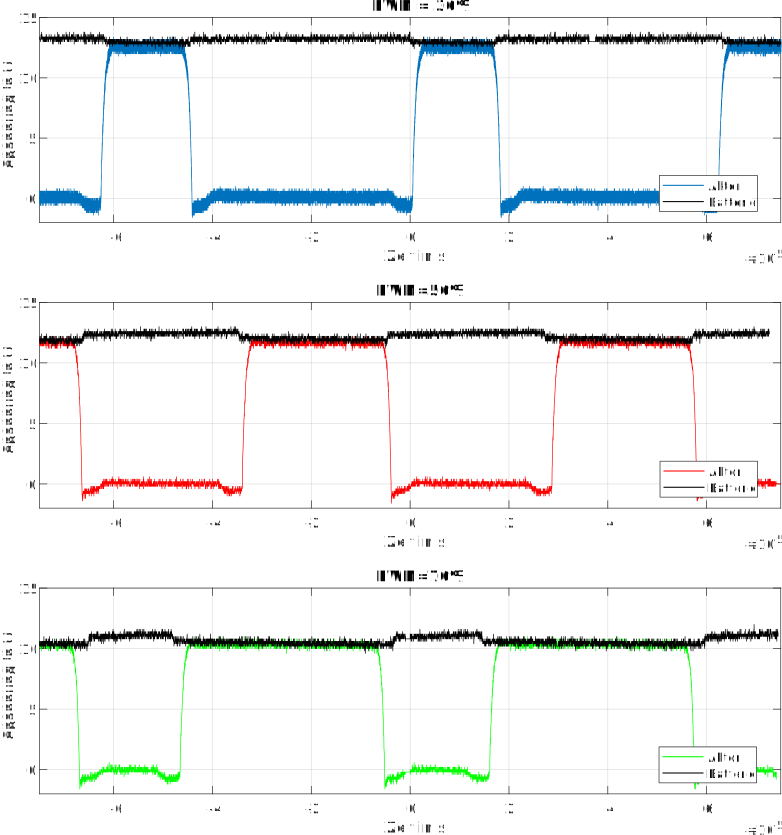
\includegraphics[width=1\linewidth]{Bilder/spannungsverlauefe.pdf}
	\caption{Spannungsverläufe an Aktor und Quelle für verschiedene PWM-Signale}
	\label{fig:spannungsverlaeufe}
\end{figure}


\chapter{Fazit und Ausblick}\label{kap8}
%%%%%%%%%%%%%%%%%%%%%%%%%%%%%%%%%%%%%%%%%%
\newpage
\pagenumbering{Roman}
\phantomsection
\addcontentsline{toc}{chapter}{Literaturverzeichnis}
\printbibliography[title=Literaturverzeichnis]

\appendix
\chapter{Vollständiges Boardlayout}\label{app:boardlayout}
\begin{figure}[H]%
\centering
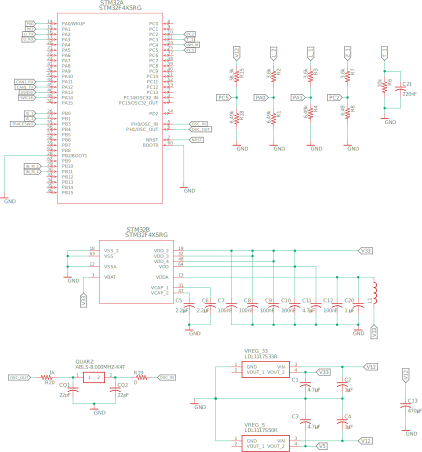
\includegraphics[angle=0,width=1
\columnwidth]{./Bilder/schem_app_1}%
\caption{Schaltplan MCU, Quarz, Spannungsregler, Spannungsteiler Sensorik}%
\label{}%
\end{figure}\newpage
\begin{figure}[H]%
\centering
\includegraphics[angle=0,width=1
\columnwidth]{./Bilder/schem_app_2}%
\caption{Schaltplan CAN-Transciever, H-Brücke, Leitungstreiber, Ausgangsblöcke, Stecker}%
\label{}%
\end{figure}\newpage
\begin{figure}[H]%
\centering
\includegraphics[angle=-90,width=0.7\columnwidth]{./Bilder/docu}%
\caption{Bauteilplatzierung des 2-Layer-Entwurfs}%
\label{}%
\end{figure}\newpage
\begin{figure}[H]%
\centering
\includegraphics[angle=-90,width=0.7\columnwidth]{./Bilder/top2}%
\caption{Top-Layer des 2-Layer-Entwurfs}%
\label{}%
\end{figure}\newpage
\begin{figure}[H]%
\centering
\includegraphics[angle=-90,width=0.7\columnwidth]{./Bilder/bottom2}%
\caption{Bottom-Layer des 2-Layer-Entwurfs}%
\label{}%
\end{figure}

\chapter{Alternativkonzept auf 4 Layern mit Buck-Converter}\label{app:4layer}
Wie in \autoref{sec:platan} beschrieben sind bisher keine Probleme durch EMI aufgetreten, sodass die Erweiterung auf ein 4-Layer Platinenlayout nur notwendig wäre, wenn in der zukünftigen Aktorkonfiguration Probleme auftreten sollen. Die Erweiterung bezieht sich hauptsächlich auf die Einführung eines Buck-Converters aus \autoref{fig:buckcon}, welcher die \SI{5}{V} Spannungsebene erzeugen könnte und die Einführung einer GND-Plane im zweiten Layer (vgl. \autoref{fig:groundplane}). Der Buck-Converter regelt auf die \SI{5}{V} über Schaltzyklen ähnlich denen eines PWM-Signals. Über die \SI{5}{V} des Buck-Converters wird der LDO für die \SI{3,3}{V} Spannungsebene gespeist, wie \autoref{fig:ldobuck} zeigt.
\begin{figure}[H]%
\centering
\includegraphics[width=0.8\columnwidth]{./Bilder/buck}%
\caption{Buck-Converter zum Regeln auf \SI{5}{V}}%
\label{fig:buckcon}%
\end{figure}\noindent
Diese Konfiguration hat den Vorteil, dass der LDO der \SI{3,3}{V} Spannungsebene weniger stark belastet wird. Problem an einem Buck-Converter ist, dass aufgrund der Schaltzyklen die Spannung weniger konstant ist, als bei einem LDO. Durch die Kombination beider Regler ist die \SI{3,3}{V} Spannungsebene so stabil wie in der vorherigen Spannungsregler-Konfiguration. Zu Analysieren wäre allerdings, wie sich der Buck-Converter auf das Auslesen der Lagesensorik auswirkt, welche von den \SI{5}{V} gespeist wird. Im derzeitigen Entwurf wurde sich deshalb für zwei seperate LDOs entschieden (vgl. \autoref{sec:spannver}).
\begin{figure}[H]%
\centering
\includegraphics[width=0.8\columnwidth]{./Bilder/v334layer}%
\caption{LDO-Converter zum Regeln auf \SI{3,3}{V} bei \SI{5}{V} Eingangsspannung}%
\label{fig:ldobuck}%
\end{figure}\noindent
Nach \cite{Franz2012} wird die GND-Plane in Layer 2 (vgl. \autoref{fig:groundplane}) eingeführt um eine Abschirmung des Top-Layers gegenüber Layer 3 und Layer 4 zu erreichen, was eine Verbesserung der EMV bezweckt. Die Signalleitungen werden so möglichst in den unteren Layern verlegt um eine gute Abschirmung zu garantieren \cite{emcdes}.
\newpage
\begin{figure}[H]%
\centering
\includegraphics[angle=-90,width=0.7\columnwidth]{./Bilder/doc4layer}%
\caption{Bauteilplatzierung des 4-Layer-Entwurfs}%
\label{}%
\end{figure}\newpage
\begin{figure}[H]%
\centering
\includegraphics[angle=-90,width=0.7\columnwidth]{./Bilder/top4layer}%
\caption{Top-Layer des 4-Layer-Entwurfs}%
\label{}%
\end{figure}\newpage
\begin{figure}[H]%
\centering
\includegraphics[angle=-90,width=0.7\columnwidth]{./Bilder/2route4layer}%
\caption{Zweites Layer des 4-Layer-Entwurfs}%
\label{fig:groundplane}%
\end{figure}\newpage
\begin{figure}[H]%
\centering
\includegraphics[angle=-90,width=0.7\columnwidth]{./Bilder/15route4layer}%
\caption{Drittes Layer des 4-Layer-Entwurfs}%
\label{}%
\end{figure}\newpage
\begin{figure}[H]%
\centering
\includegraphics[angle=-90,width=0.7\columnwidth]{./Bilder/bot4layer}%
\caption{Bottom-Layer des 4-Layer-Entwurfs}%
\label{}%
\end{figure}\newpage


\end{document}
